\documentclass[10pt]{article}
\usepackage[utf8]{inputenc}
\usepackage{amsmath, amsthm, amssymb}
\usepackage{graphicx}
\usepackage{caption}
\captionsetup[figure]{skip=4pt}  % padrão ~10pt, pode reduzir aqui
\usepackage{float}
\usepackage{geometry}
\usepackage{setspace}
\usepackage{url}
\usepackage[alf]{abntex2cite}
\bibliographystyle{abntex2-alf}  % ou abntex2-num
\usepackage{indentfirst}
\usepackage{enumitem}
\geometry{a4paper, margin=2.5cm}
\setstretch{1.2}
\usepackage{listings}
\usepackage{xcolor} % Para cores
\usepackage{booktabs}  % Tabelas mais elegantes
\usepackage{siunitx}   % Alinhamento numérico opcional



\lstdefinestyle{python}{
    language=Python,
    basicstyle=\ttfamily\small,
    keywordstyle=\color{blue},
    stringstyle=\color{red},
    commentstyle=\color{gray},
    showstringspaces=false,
    frame=single,
    breaklines=true
}

\lstdefinestyle{gnuplot}{
    language=sh, % ou bash (não há suporte nativo direto a gnuplot)
    basicstyle=\ttfamily\small,
    commentstyle=\color{gray},
    keywordstyle=\color{blue},
    stringstyle=\color{red},
    showstringspaces=false,
    breaklines=true,
    frame=single
}

\title{\bfseries Primeira lista de exercícios}
\author{Edison Ribeiro Araújo - RA : 24202520836}
\date{\today}

\begin{document}

        \maketitle
        
\begin{abstract}

\noindent
Este trabalho é a lista de exercícios do professor Saul Leite da turma 202502 de Métodos Numéricos.
Lista referente a Séries de Taylor, Resíduos e Horner.
\vspace{2em}
\end{abstract}

        \section{Exercício 1}

Encontre o polinômio de Taylor de grau 1, 2, 3, e 4 para a função $ f(x) = log(5+6x) $,
expandindo em torno de $X_0 = 0$. Usando Python, faça os gráficos dos polinômios e da
função.


        \subsection{Resultado - Exercício 1}

Os passos são:
\begin{itemize}[leftmargin=3.5em, itemsep=-.5mm, topsep=0.5mm]
    \item Derivar f(x) 4 vezes.
    \item Aplicar a série de Taylor
    \item Gerar dados em Pyhon
    \item Imprimir Gráfico usando GnuPlot
    \item Apresentar o código Python e GnuPlot
 \end{itemize}

\subsubsection{Derivar f(x) 4 vezes}

derivar a função $f(x) = \log(5 + 6x)$ usando a regra da cadeia.
Primeiro, identificamos as funções internas:

\[
    \begin{aligned}
        f(g(x)) &= \log(5 + 6x) \\
        f(x) &= \log(x) \\
        g(x) &= 5 + 6x
    \end{aligned}
\]

Aplicamos a regra da cadeia:

\[
    \frac{d}{dx} f(g(x)) = f'(g(x)) \cdot g'(x)
\]

Calculamos as derivadas individuais:

\[
    \begin{aligned}
        f(x) &= \log(x) \\
        f'(x) &= \frac{1}{x} \\
        g(x) &= 5 + 6\cdot x \\
        g'(x) &= 6
    \end{aligned}
\]

Substituindo na regra da cadeia:

\[
    \frac{d}{dx} f(g(x)) = \frac{1}{5 + 6x} \cdot 6 = \frac{6}{5 + 6x}
\]

Portanto, a derivada da função é:

\[
    f'(x) = \frac{6}{5 + 6x}
\]
Aplicamos a derivada mais uma vez:

\[
    \begin{aligned}
        f''(x) = 6 * \frac{d}{dx} (5 + 6x)^{-1} \\
        f''(x) = - 6 * 6 *  \frac{1}{ (5 + 6x)^{2} } \\
        f''(x) = - \frac{36}{ (5 + 6x)^{2} } \\
    \end{aligned}
\]

Repetindo o processos temos:

\[
    \begin{aligned}
        f'''(x) = \frac{d}{dx} -\frac{36}{(5 + 6x)^{2}} \\
        f'''(x) = - 36 \cdot \frac{d}{dx} (5 + 6x)^{-2} \\
        f'''(x) = 36 \cdot 6 \cdot 2 \cdot (5 + 6x)^{-3} \\
        f'''(x) = 432 \cdot (5 + 6x)^{-3} \\
        f'''(x) = \frac{432}{ (5 + 6x)^{3} } \\
    \end{aligned}
\]

Fazendo a última derivada:

\[
    \begin{aligned}
        f''''(x) =\frac{d}{dx} \frac{432}{ (5 + 6x)^{3} }\\
        f''''(x) = 432 \cdot \frac{d}{dx} \cdot (5 + 6x)^{-3}\\
        f''''(x) = -3 \cdot 6 \cdot 432 \cdot (5 + 6x)^{-4}\\
        f''''(x) = -7776 \cdot (5 + 6x)^{-4}\\
        f''''(x) = \frac{-7776}{(5 + 6x)^{4}}\\
    \end{aligned}
\]

\subsubsection{Aplicar a série de Taylor}

Agora com as derivadas em mãos:

\[
    \begin{aligned}
        f'(x) =    \frac{6}{5 + 6x} \\
        f''(x) =   \frac{-36}{ (5 + 6x)^{2} } \\
        f'''(x) =  \frac{432}{ (5 + 6x)^{3} } \\
        f''''(x) = \frac{-7776}{(5 + 6x)^{4}}\\
    \end{aligned}
\]

Podemos aplicar a Série de Taylor.
\[
    f(x) = \sum_{n=0}^{\infty} \frac{f^{(n)}(x_0)}{n!}(x - x_0)^n
\]

Vamos avaliar o valor em $X_0 = 0$ para cada uma das derivadas.
    \begin{gather*}
        f(0) =    \log(5) = 1.6094 \\
        f'(0) =    \frac{6}{5} \\
        f''(0) =   \frac{-36}{5^{2}}  = \frac{-36}{25} \\
        f'''(0) =  \frac{432}{5^{3}}  = \frac{432}{125} \\
        f''''(0) = \frac{-7776}{5^{4}} = \frac{-7776}{625} \\
    \end{gather*}

Montando as Séries temos:
    \begin{gather*}
        P_0 (x) = f(0) = \log(5) = 1.6094\\
        P_1 (x) = P_0(x) + \frac{\frac{6}{5}}{1!} \cdot x = P_0(x) + \frac{6 \cdot x}{5} \\
        P_2 (x) = P_1(x) + \frac{\frac{-36}{25}}{2!} \cdot x^2 = P_1(x) + \frac{-36 \cdot x^2}{50} \\
        P_3 (x) = P_2(x) + \frac{\frac{432}{25}}{3!} \cdot x^3 = P_2(x) + \frac{432 \cdot x^3}{150} \\
        P_4 (x) = P_3(x) + \frac{\frac{7776}{625}}{4!} \cdot x^3 = P_3(x) + \frac{-7776 \cdot x^4}{15000} \\
    \end{gather*}

\subsubsection{Gerar dados em Pyhon}

Com todos os coeficientes do polinômio podemos codificar e executando o programa em Python com o comando para criar o arquivo com os dados: python exercicio1.py

%%\newpage

\subsubsection{Imprimir Gráfico usando GnuPlot}

Agora com todas as funções definidas, e dados gerados podemos gerar o gráfico para visualizar as diferenças:

\begin{figure}[htbp]
    \centering
    \includegraphics[width=.82\textwidth]{imagens/exercicio1.png}
    \caption{Função $\log(5+6*x)$ aproximada pelo série de taylor em torno de $X_0=0$}
    \label{fig:grafico}
\end{figure}

\newpage

\subsubsection{Apresentar código Python e GnuPlot}

\lstinputlisting[style=python]{scripts/exercicio1.py}
Código para a geração dos dados no arquivo exercício1.csv
\newpage

\lstinputlisting[style=gnuplot]{scripts/exercicio1.gnuplot}
Código para do gráfico do exercício1 baseado nos dados do arquivo exercício1.csv

\newpage







        \section{Exercício 2}

Use os polinômios de Taylor para mostrar que $(1 + t)^n = \sum_{j=0}^{n} \binom{n}{j} t^j$, para $n$ inteiro e maior do que 1, \\
e onde $\binom{n}{j} = \dfrac{n!}{(n - j)! j!}$ é o coeficiente binomial.





        \subsection{Resultado - Exercício 2}

Os passos são:
\begin{itemize}[leftmargin=3.5em, itemsep=-.5mm, topsep=0.5mm]
    \item Derivar $f^{(k)}(t)$ de forma genérica
    \item Descobrir quanto vale $f^{(k)}(0)$ de forma genérica.
    \item Expandir para a Série de taylor para forma genérica
    \item Gerar tabela para comparação
    \item Apresentar o código Python
 \end{itemize}

\subsubsection{Derivar $f^{(k)}(t)$ de forma genérica}

\begin{figure}[H]
    \centering
    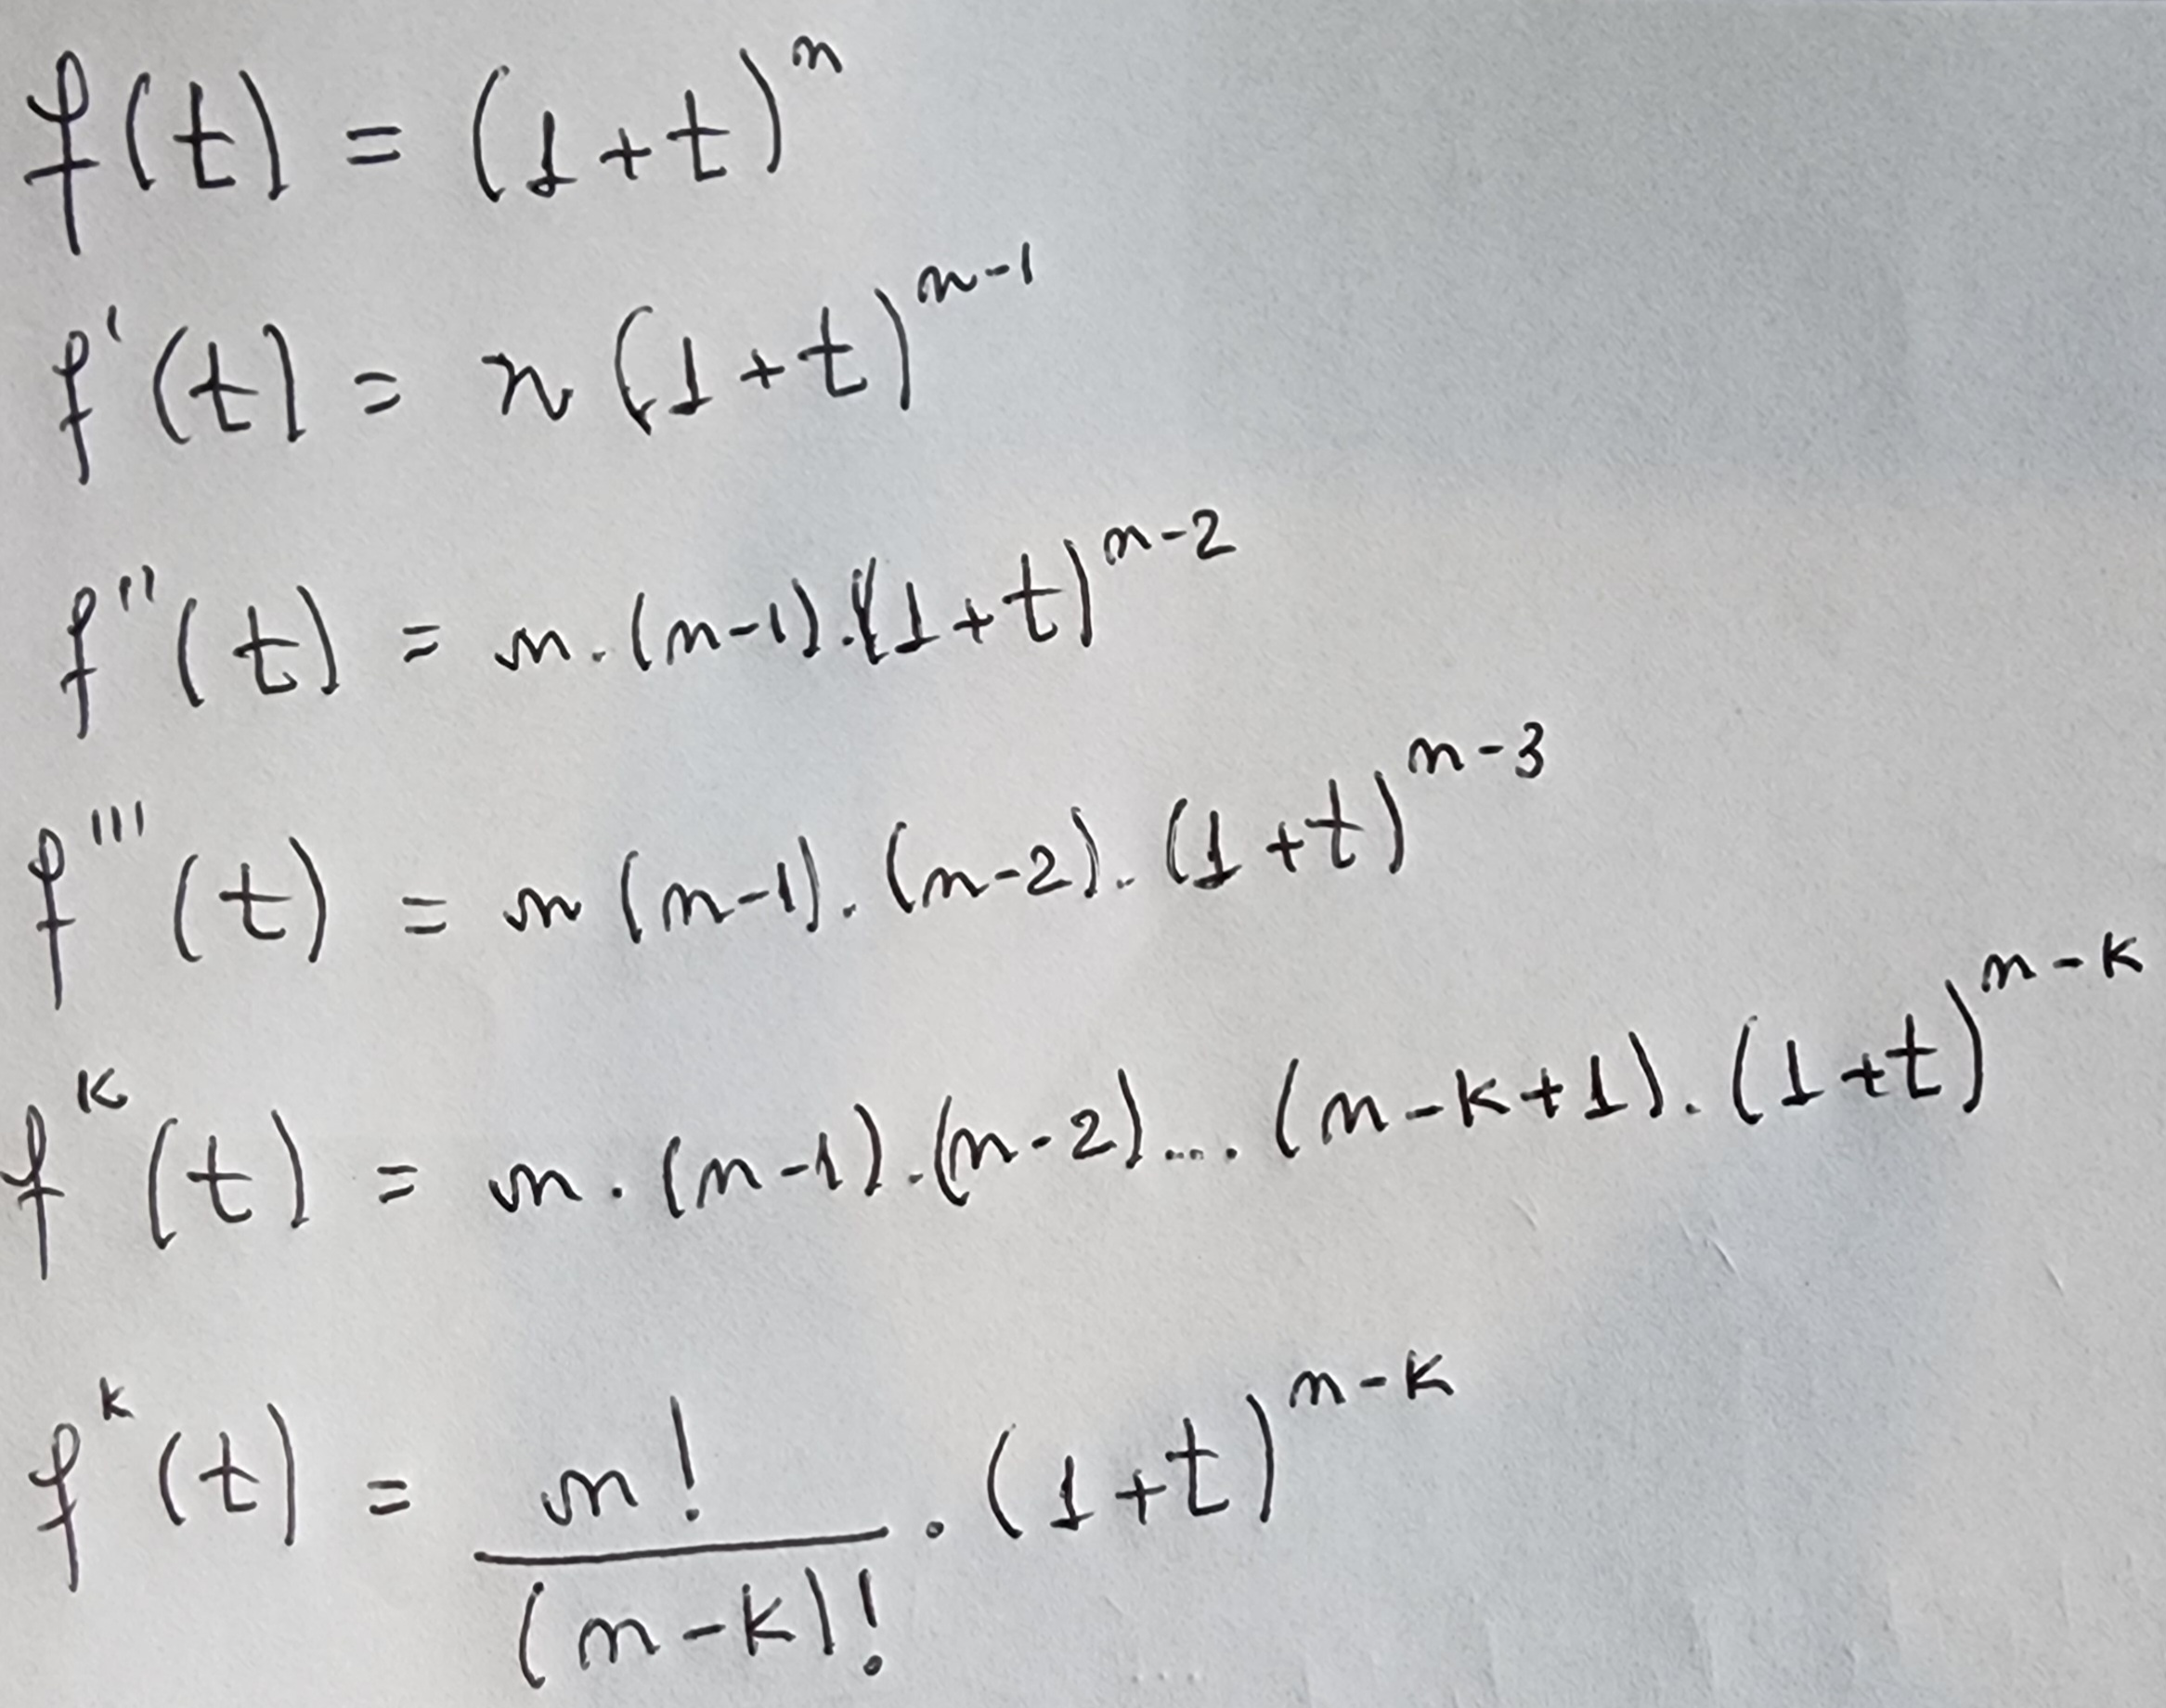
\includegraphics[width=1.0\textwidth]{imagens/exercicio2_parte1}
    \caption{Calculando as derivadas de $f(t)$ como resultado $f^{(k)}(t) = \frac{n!}{(n-k)!} \cdot (1 + t)^{n-k}$}
    \label{fig:exe2_parte1}
\end{figure}

\subsubsection{Descobrir quanto vale $f^{(k)}(0)$ de forma genérica.}
\begin{figure}[H]
    \centering
    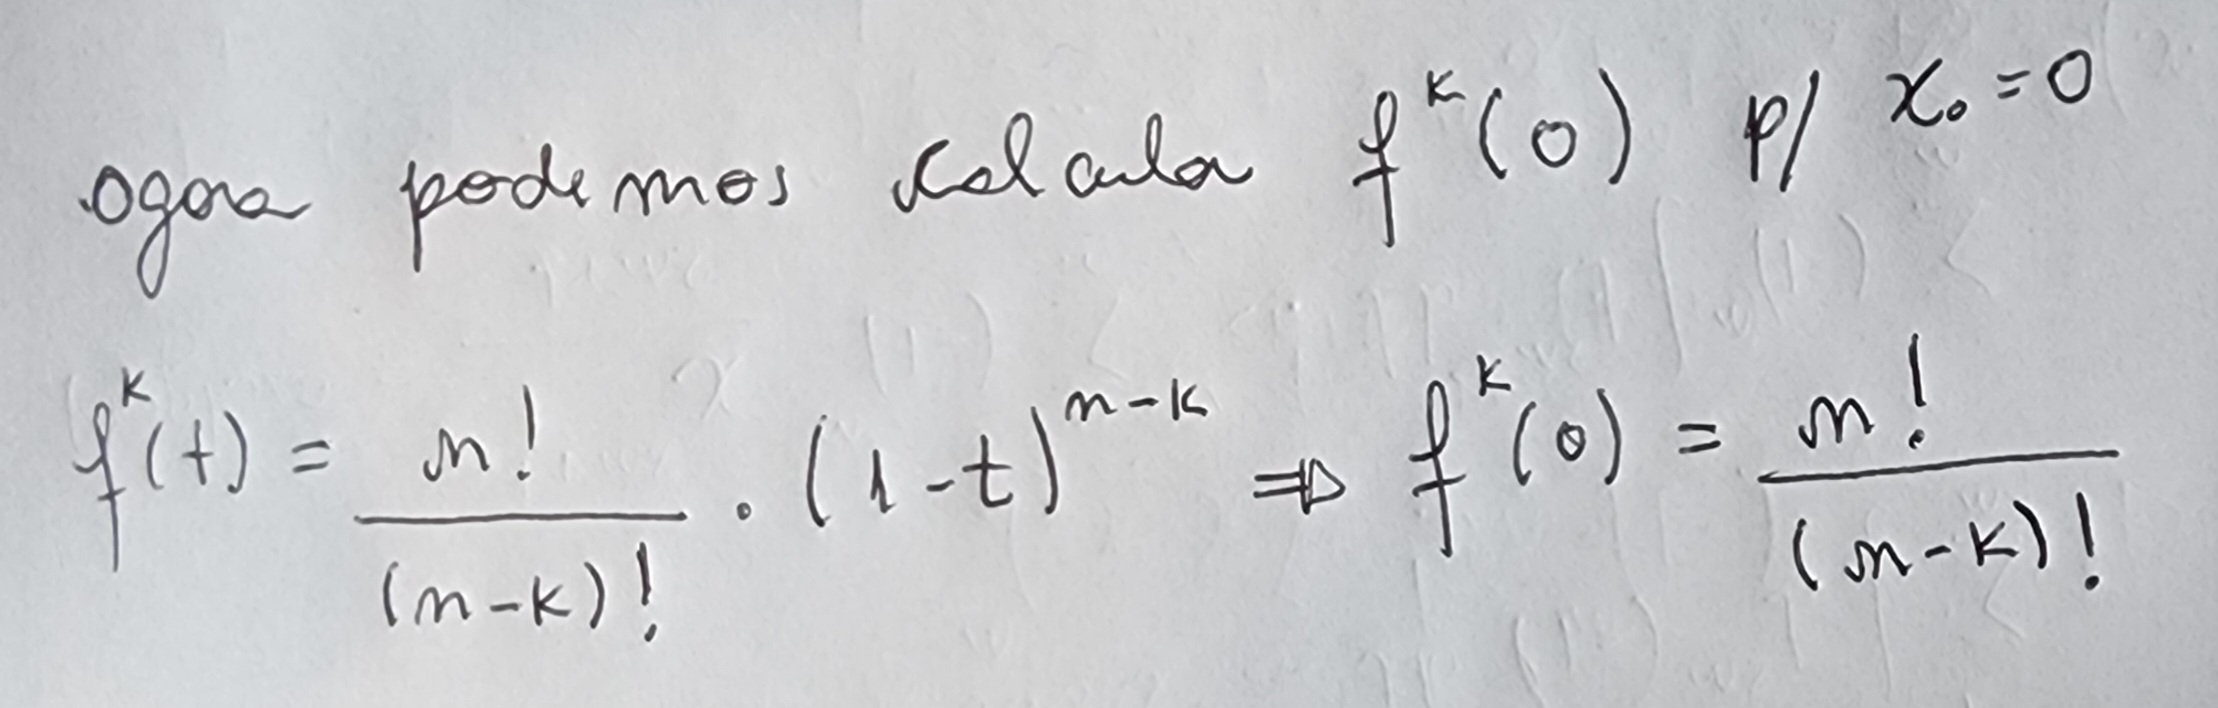
\includegraphics[width=1.0\textwidth]{imagens/exercicio2_parte2}
    \caption{Calculando $f^{(k)}(t)$ para $t = x_0 = 0$}
    \label{fig:exe2_parte2}
\end{figure}

\subsubsection{Expandir para a Série de taylor para forma genérica}
\begin{figure}[H]
    \centering
    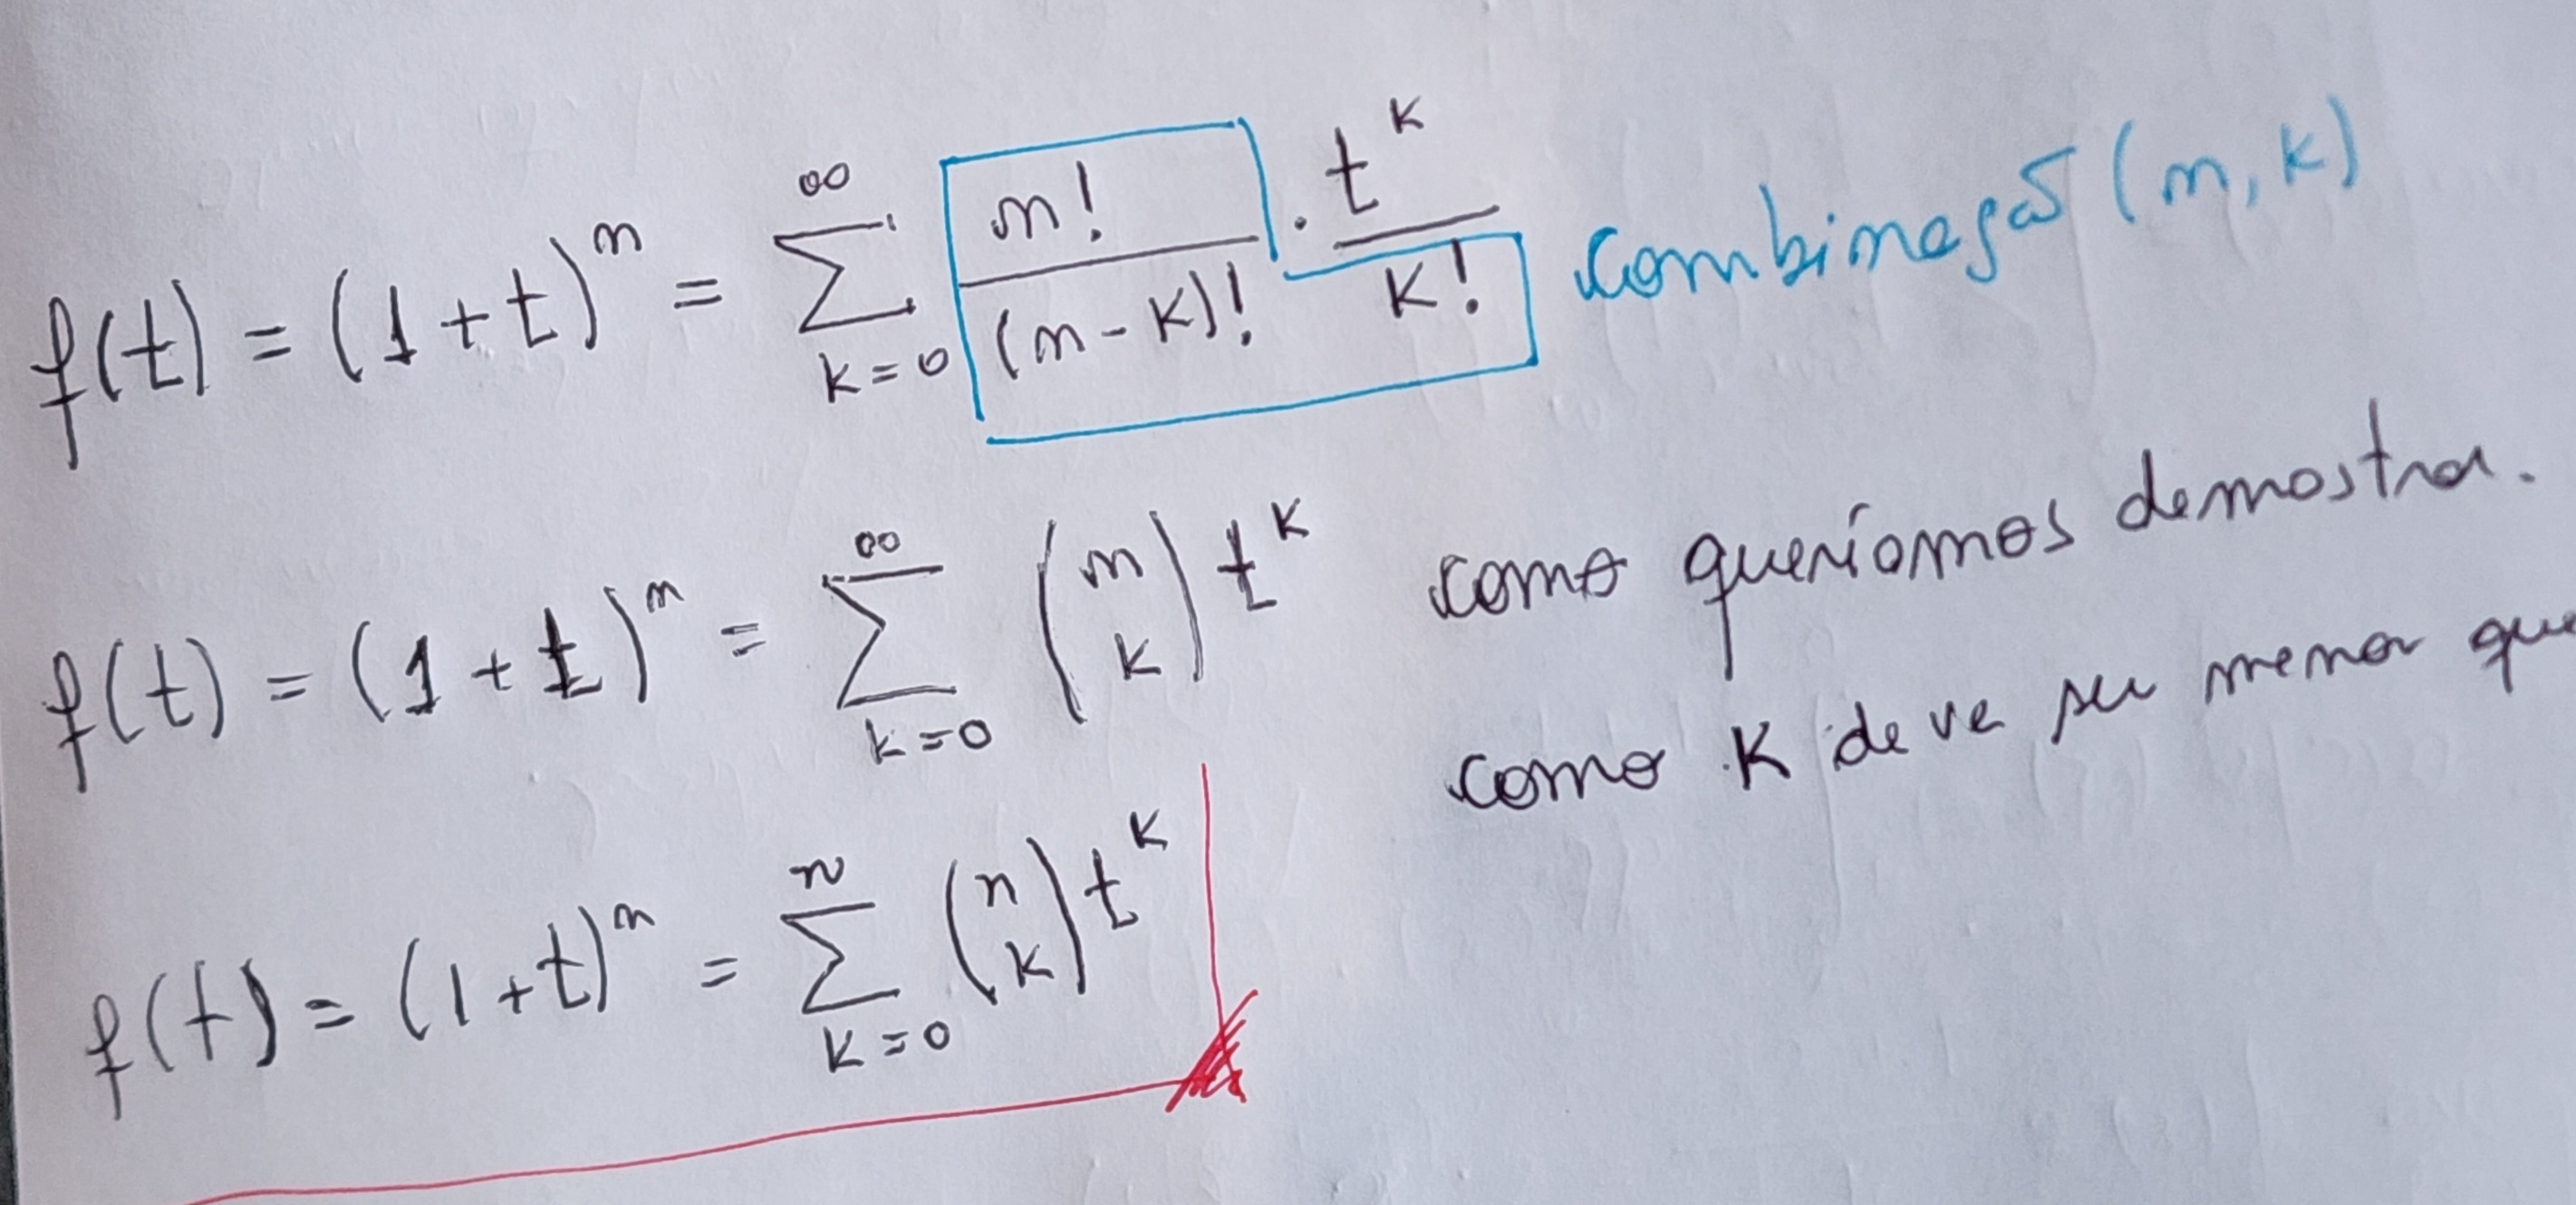
\includegraphics[width=1.0\textwidth]{imagens/exercicio2_parte3}
    \caption{Calculando $f(t)$ em para $t = x_0 = 0$ usando a Série de Taylor comprovando o enunciado.}
    \label{fig:exe2_parte3}
\end{figure}
Como k não pode ser maior que n, a última linha mostra que limitamos k entre 0 e n e não mais entre 0 e $\infty$

\subsubsection{Gerar tabela para comparação}

    \begin{table}[H]
    \centering
    \caption{Testes do Exercicio 2 com n = 10.}
    \label{tab:exercicio_2_resultados}
    \begin{tabular}{|c|c|c|c|}
    \toprule
    \textbf{$x$} & \textbf{$f(x,10)$} & \textbf{$P_k(x,10)$} & \textbf{Diferenca} \\
    \midrule   
    -1.0000e+01 & 3.4868e+09 & 3.4868e+09 & 0.0000000e+00 \\
                            -9.0000e+00 & 1.0737e+09 & 1.0737e+09 & 0.0000000e+00 \\
                            -8.0000e+00 & 2.8248e+08 & 2.8248e+08 & 0.0000000e+00 \\
                            -7.0000e+00 & 6.0466e+07 & 6.0466e+07 & 0.0000000e+00 \\
                            -6.0000e+00 & 9.7656e+06 & 9.7656e+06 & 0.0000000e+00 \\
                            -5.0000e+00 & 1.0486e+06 & 1.0486e+06 & 0.0000000e+00 \\
                            -4.0000e+00 & 5.9049e+04 & 5.9049e+04 & 0.0000000e+00 \\
                            -3.0000e+00 & 1.0240e+03 & 1.0240e+03 & 0.0000000e+00 \\
                            -2.0000e+00 & 1.0000e+00 & 1.0000e+00 & 0.0000000e+00 \\
                            -1.0000e+00 & 0.0000e+00 & 0.0000e+00 & 0.0000000e+00 \\
                            0.0000e+00 & 1.0000e+00 & 1.0000e+00 & 0.0000000e+00 \\
                            1.0000e+00 & 1.0240e+03 & 1.0240e+03 & 0.0000000e+00 \\
                            2.0000e+00 & 5.9049e+04 & 5.9049e+04 & 0.0000000e+00 \\
                            3.0000e+00 & 1.0486e+06 & 1.0486e+06 & 0.0000000e+00 \\
                            4.0000e+00 & 9.7656e+06 & 9.7656e+06 & 0.0000000e+00 \\
                            5.0000e+00 & 6.0466e+07 & 6.0466e+07 & 0.0000000e+00 \\
                            6.0000e+00 & 2.8248e+08 & 2.8248e+08 & 0.0000000e+00 \\
                            7.0000e+00 & 1.0737e+09 & 1.0737e+09 & 0.0000000e+00 \\
                            8.0000e+00 & 3.4868e+09 & 3.4868e+09 & 0.0000000e+00 \\
                            9.0000e+00 & 1.0000e+10 & 1.0000e+10 & 0.0000000e+00 \\
                            1.0000e+01 & 2.5937e+10 & 2.5937e+10 & 0.0000000e+00 \\
                            
    \bottomrule
    \end{tabular}
    \end{table}    
    
\newpage

\subsubsection{Apresentar o código Python}
\lstinputlisting[style=python]{scripts/exercicio2.py}
Código para testar a solução do exercício 2.




        \section{Exercício 3}


Usando a linguagem Python, criar uma função para calcular $f(x) = \sin(x)$ 
utilizando um polinômio de Taylor em torno de $x_0 = 0$. 
O polinômio deve ter o menor grau possível de modo que o erro da aproximação seja inferior 
a $10^{-7}$ para \textit{qualquer valor} de $x \in \mathbb{R}$. 
Você precisa calcular o número de termos para a sua aproximação utilizando o Teorema de Taylor. 
Teste sua função calculando os valores para $x = \dfrac{9\pi}{4}$, $\dfrac{21\pi}{4}$ e $\dfrac{41\pi}{4}$.\linebreak

\vspace{0.1em}

(\textit{Dica:} note que a função é periódica e portanto o valor de $x$, argumento da sua função, pode ser transformado antes de operar o polinômio. Além disso, você pode calcular valores para comparação usando a função \texttt{sin} da biblioteca \texttt{numpy}.)




        \subsection{Resultado - Exercício 3}

Os passos são:
\begin{itemize}[leftmargin=3.5em, itemsep=-.5mm, topsep=0.5mm]
    \item Transformar sin(x) em série.
    \item Aplicar a fórmula do resíduo e definir o tamanho da série
    \item Imprimir a função na forma de série e usando numpy no python
    \item Realizar os testes
    \item Apresentar o código Python e GnuPlot
 \end{itemize}

\subsubsection{Transformar $sin(x)$ em série.}
Temos os cálculos para escrever $sin(x)$ usando a Série de Taylor.
\begin{figure}[H]
    \centering
    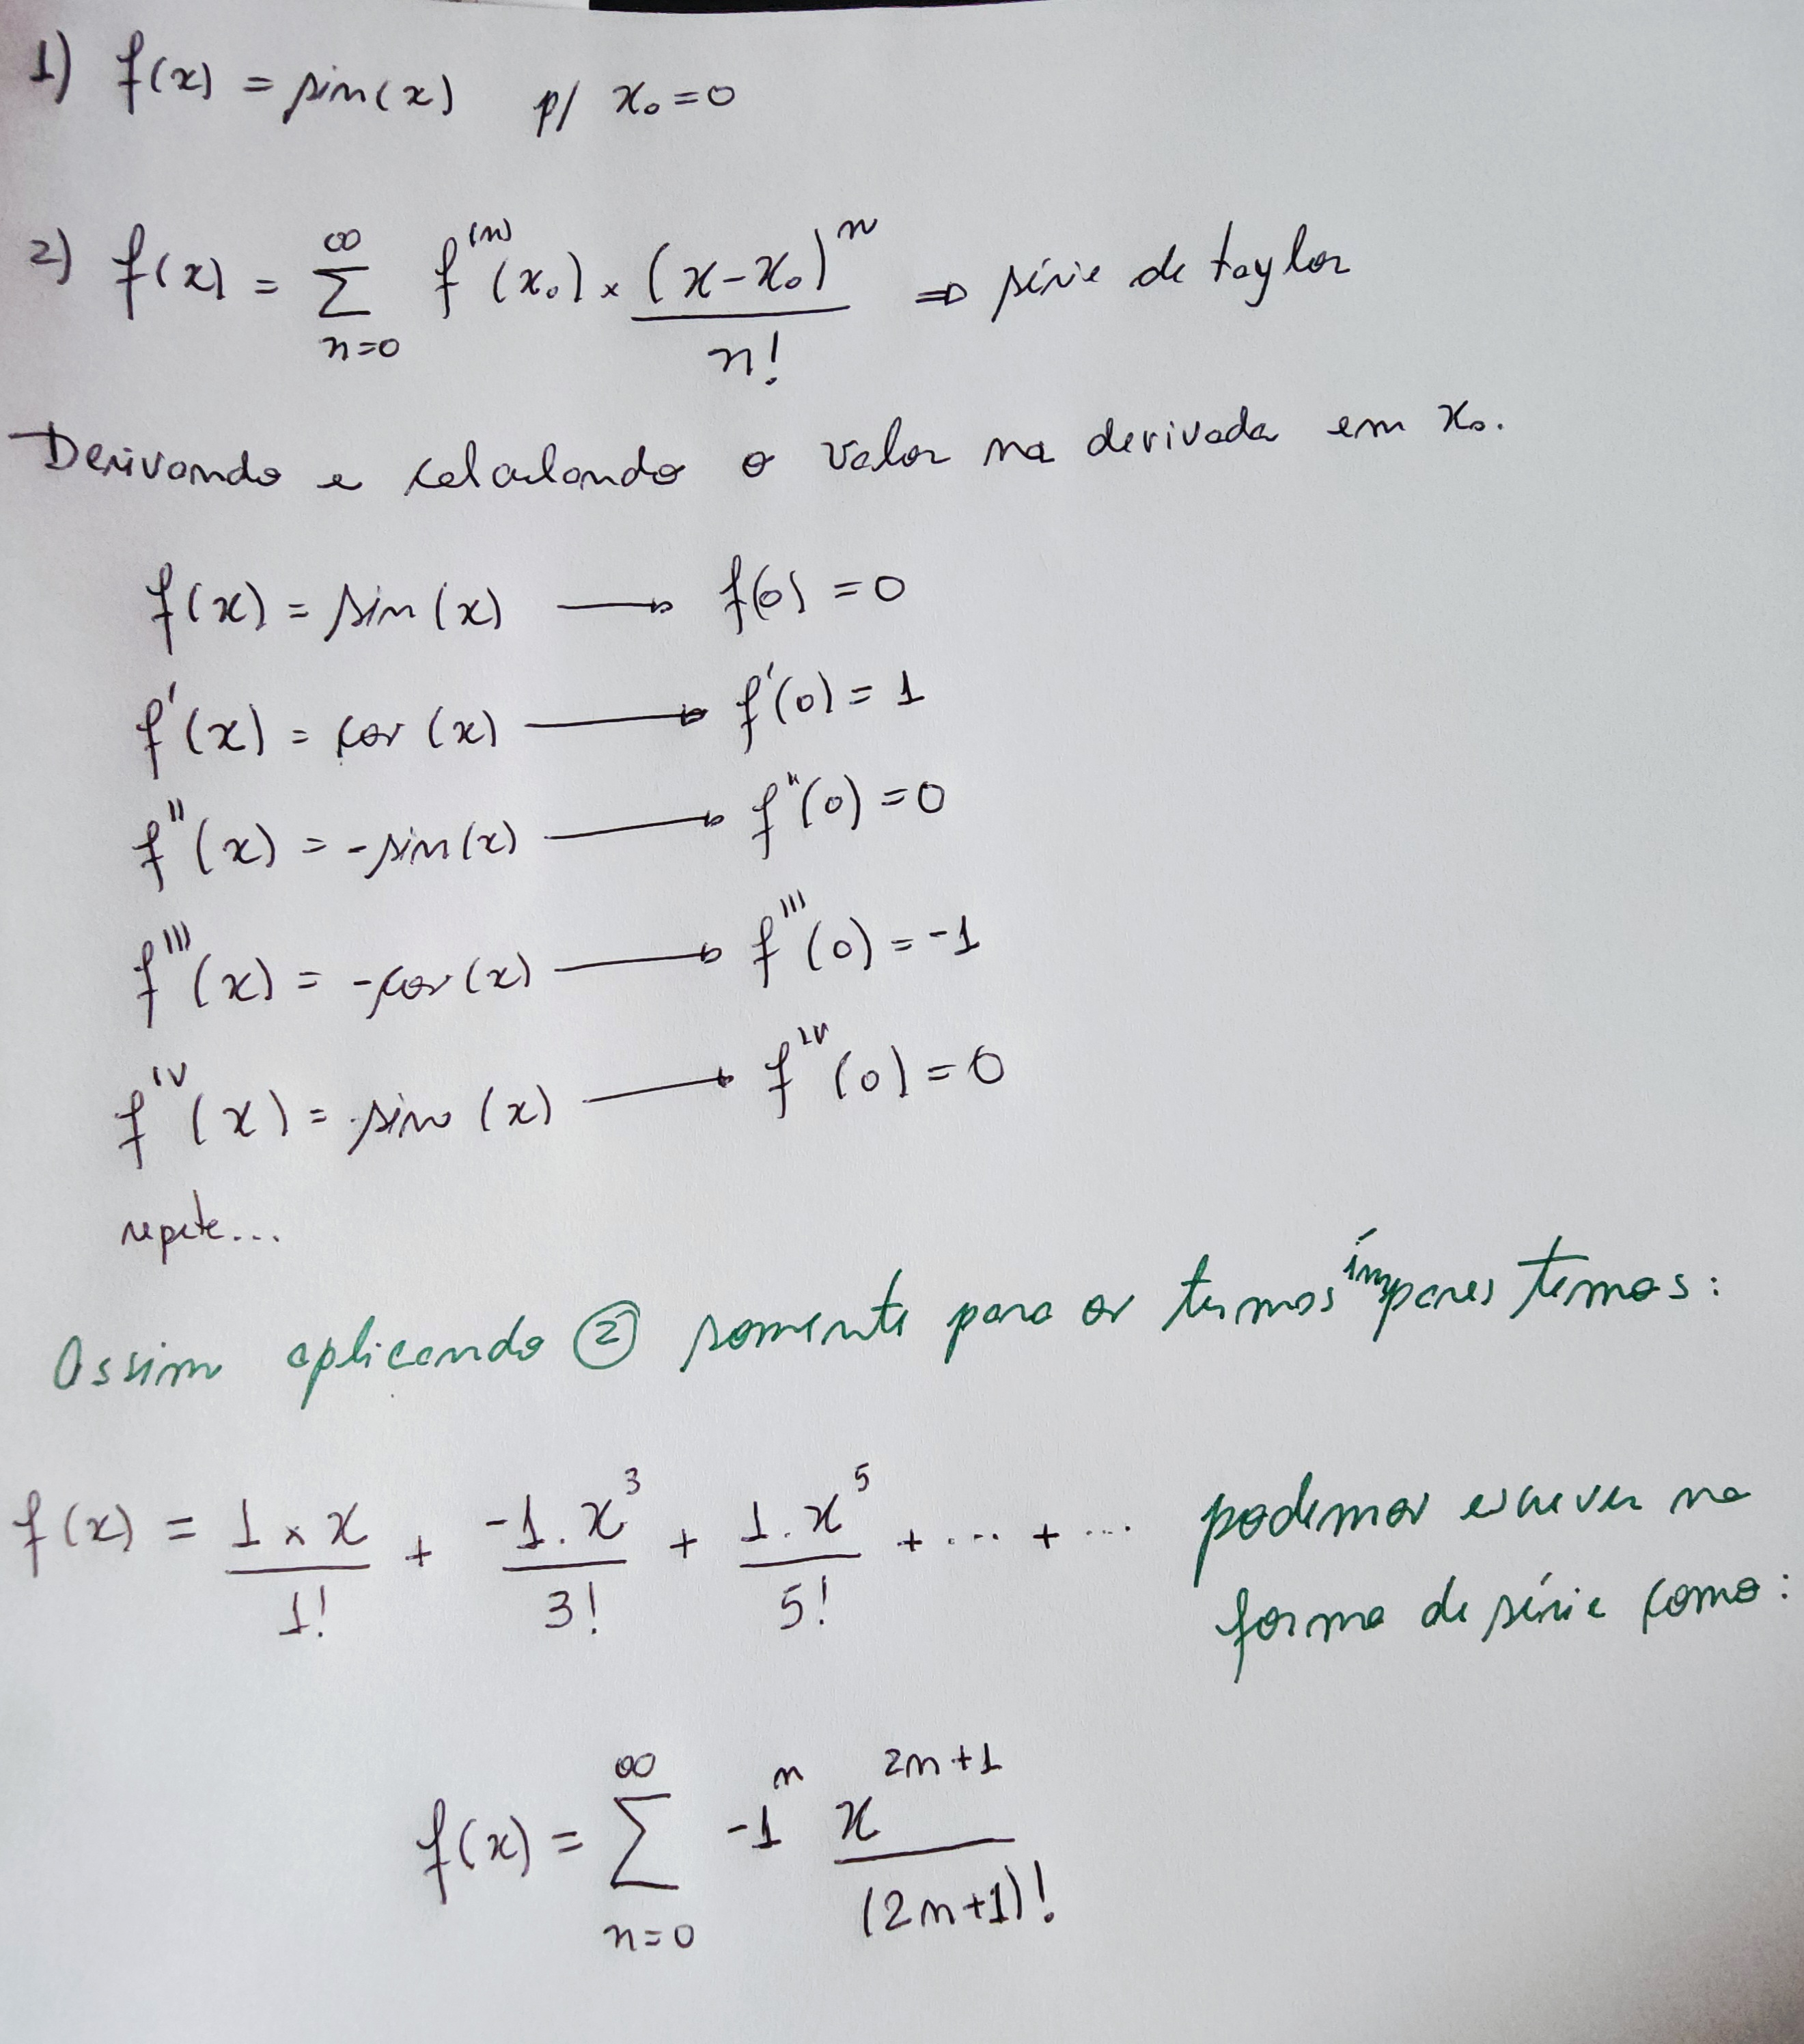
\includegraphics[width=.47\textwidth]{imagens/exercicio3_parte_1}
    \caption{Escrevendo $sin(x)$ na forma de série entre $0$ e $\frac{\pi}{2}$ obtemos como resultado $\sum_{n=0}^{\infty} -1^n \frac{x^{2 \cdot n + 1}}{(2 \cdot n + 1)!} $}
    \label{fig:lista_exercicio3_parte1}
\end{figure}
\newpage

\subsubsection{Aplicar a fórmula do resíduo e definir o tamanho da série}
Aplicando as Equações de resíduo de Taylor e o valor médio para integrais ponderadas temos:
\begin{figure}[H]
    \centering
    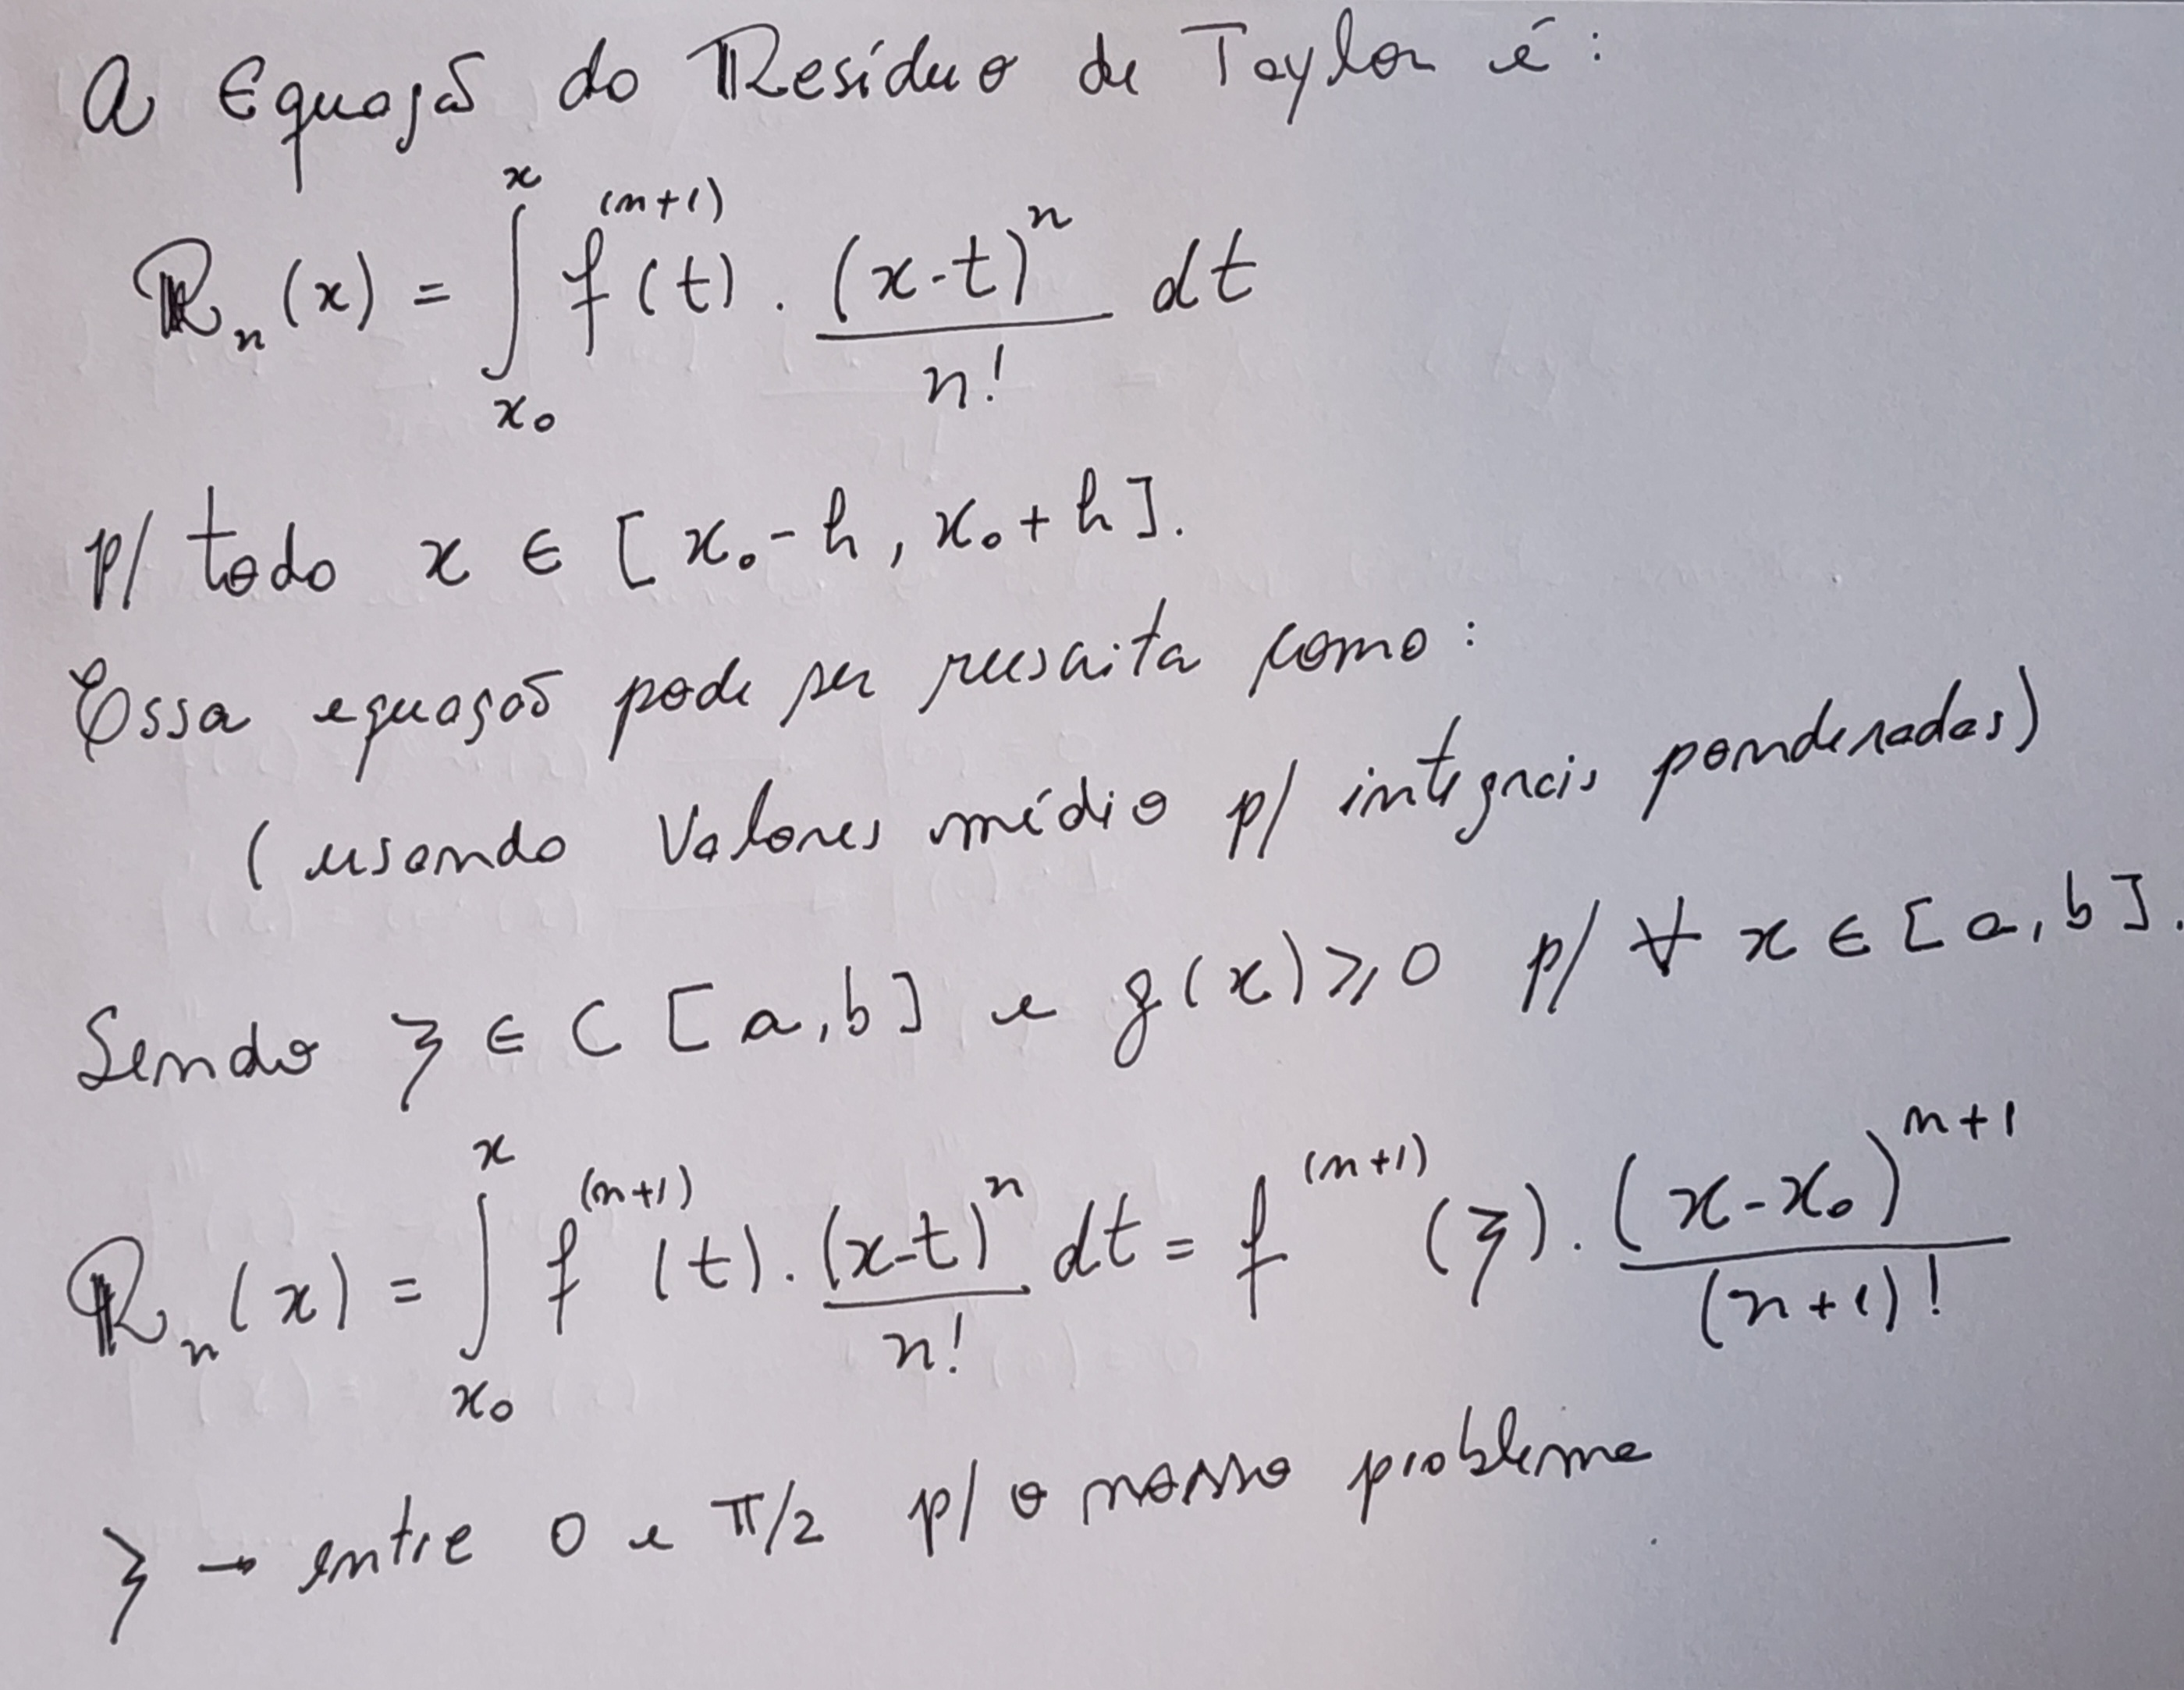
\includegraphics[width=.80\textwidth]{imagens/exercicio3_parte_2}
    \caption{Escrevendo o resíduo}
    \label{fig:lista_exercicio3_parte2}
\end{figure}
Continuando o raciocício e aplicando o resultado do resíduo.
\begin{figure}[H]
    \centering
    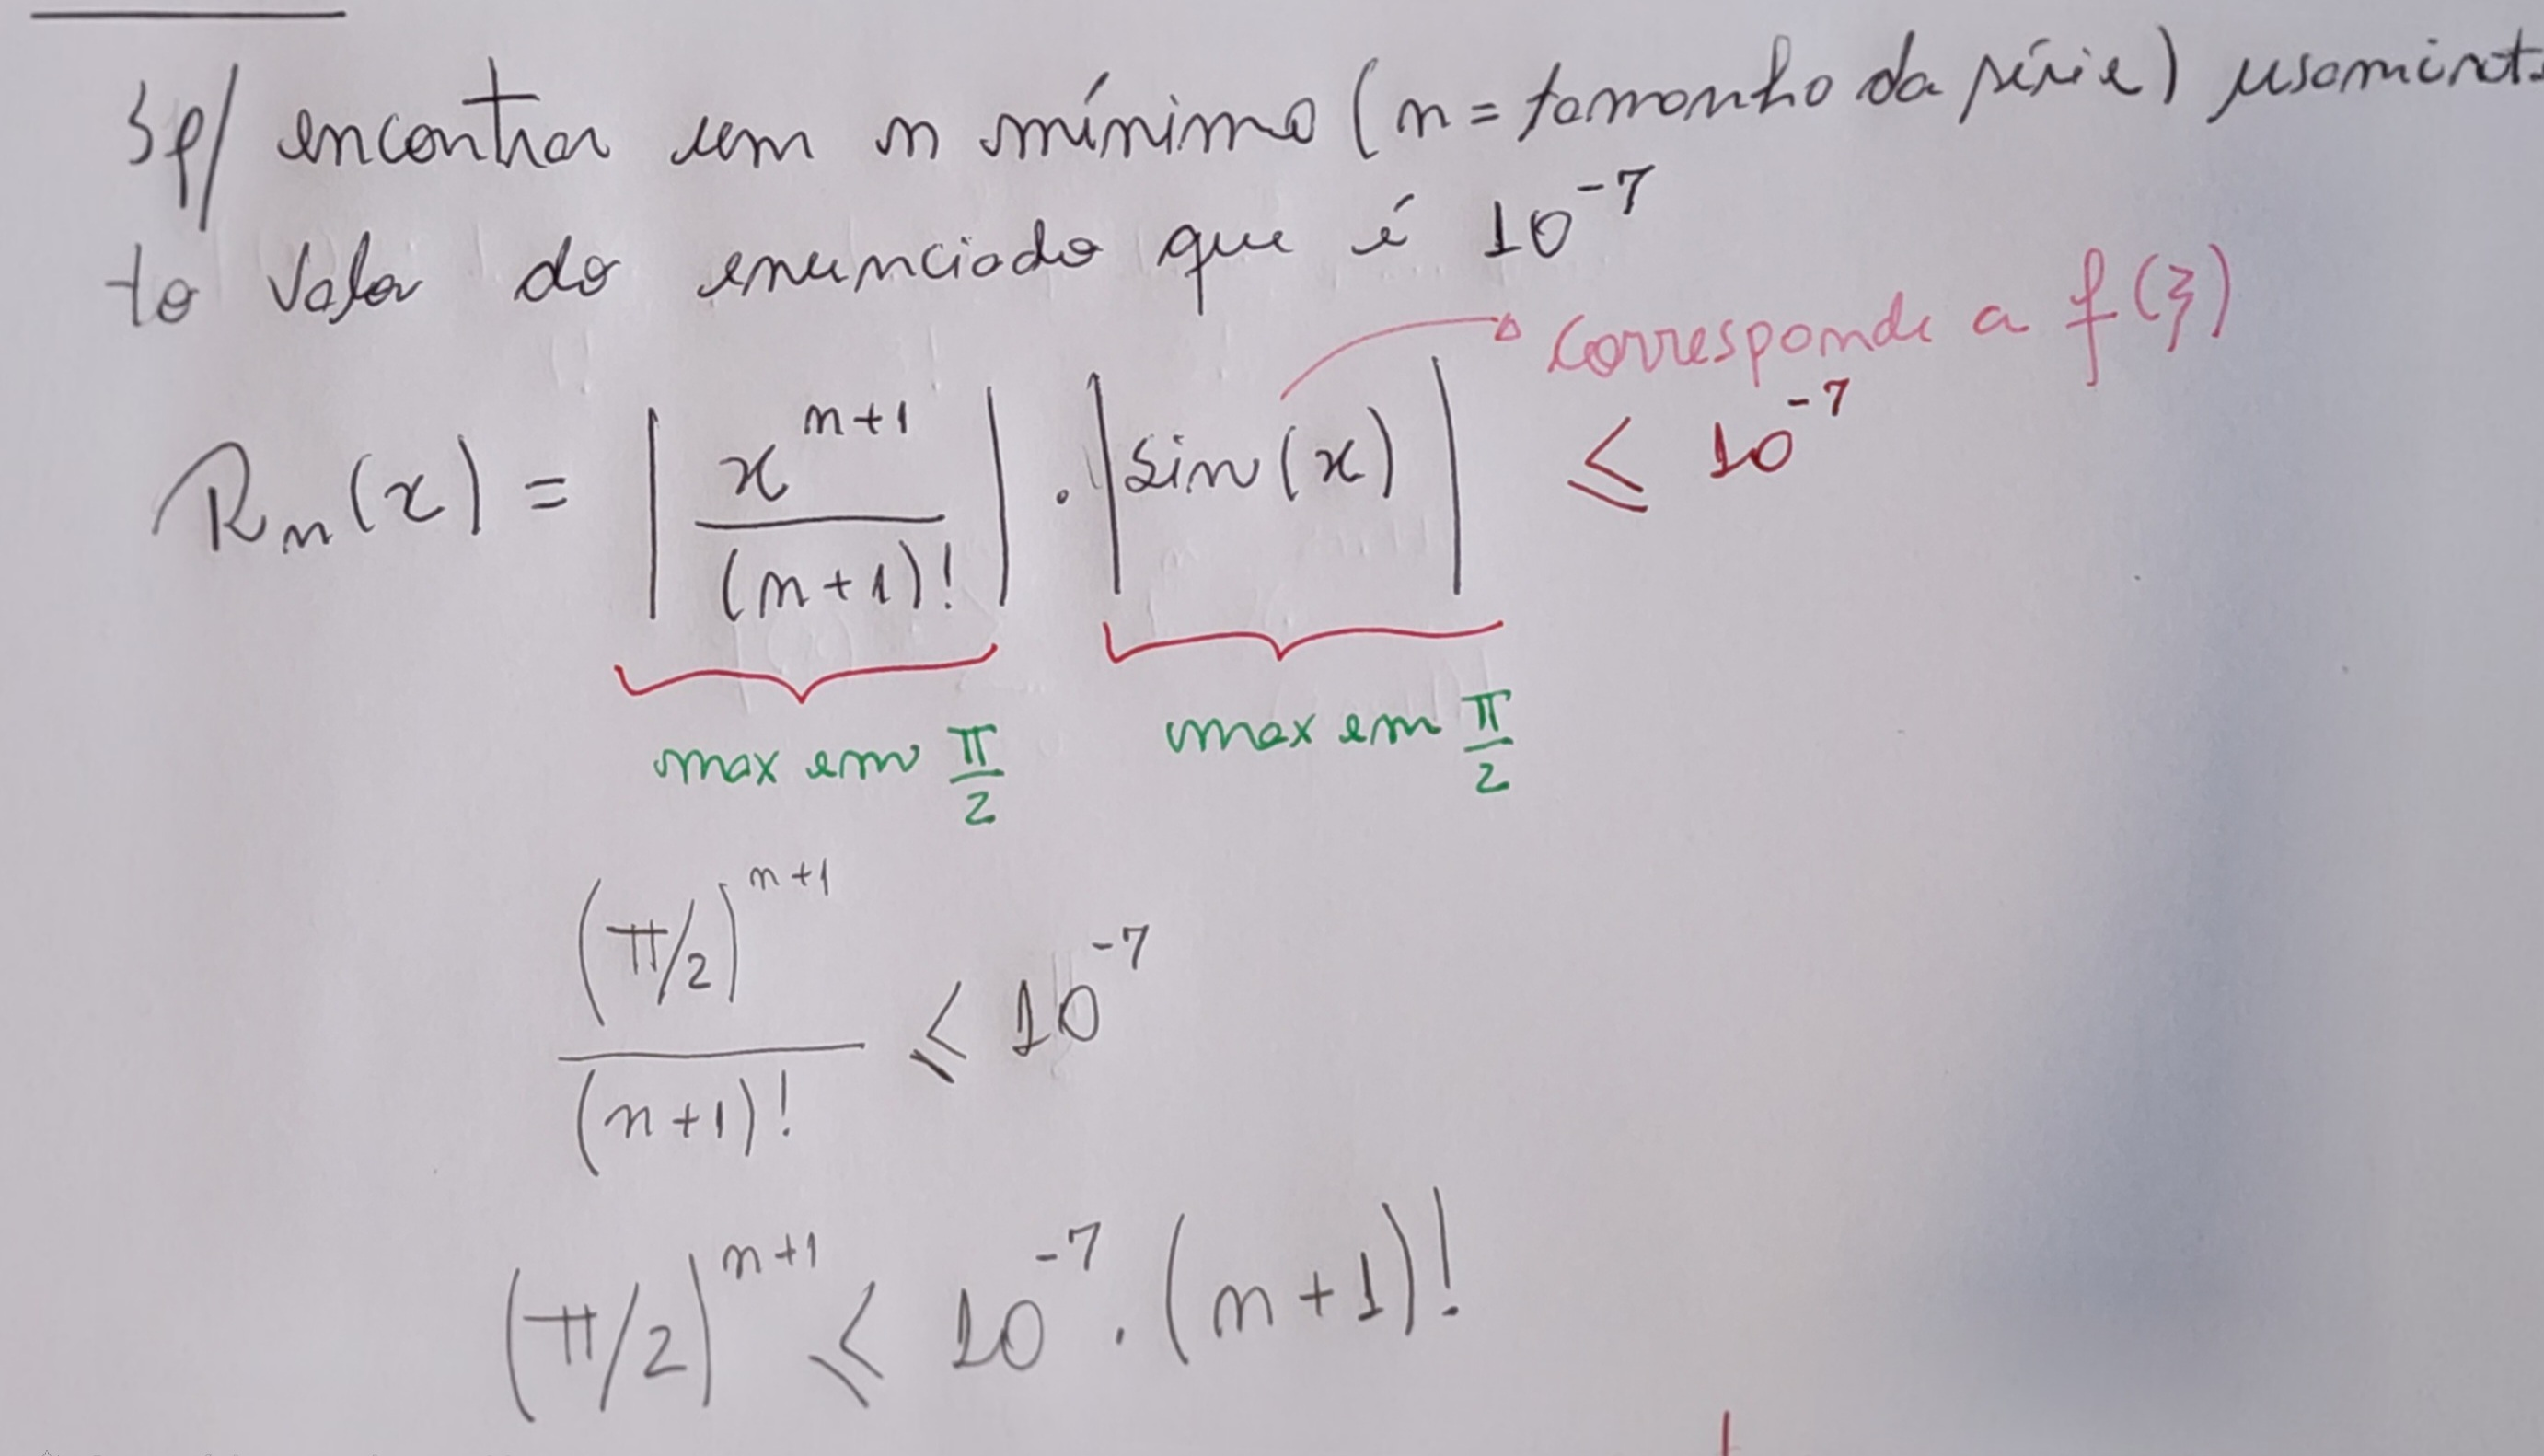
\includegraphics[width=.80\textwidth]{imagens/exercicio3_parte_3}
    \caption{Definindo a equação parar encontrar o valor de N. Essa equação foi testada com valores maiores que 2 e encontramos como verdadeiro o valor 13}
    \label{fig:lista_exercicio3_parte3}
\end{figure}

\input{tabela_residuos_exercicio3}

Usando a tabela Tabela~\ref{tab:exercicio_3_definir_grau_minimo} podemos ver que o menor grau que polinômio deve ter é 13. \\
Assim vamos definir 13 na chamada da função \texttt{calculaFTaylor} limitando o maior grau do polinômio em $\frac{x^{13}}{13!}$.

\subsubsection{Imprimir a função na forma de série e usando numpy no python}

Podemos ver nos gráficos da figura \ref{fig:grafico_exe3} que a diferença dos valores entre $-3 \cdot \pi$ a $3 \cdot \pi$ tem erros na ordem de $10^{-9}$ e que eles são maiores quando $ x = \frac{(2 \cdot n + 1)}{2} \cdot \pi $ para qualquer valor de n inteiro.
\begin{figure}[H]
    \centering
    \includegraphics[width=.95\textwidth]{imagens/exercicio3.png}
    \caption{Gráfico da função seno gerada por numpy , $P_3(x)$ e $P_{13}(x)$ e o módulo da diferença de $F(x)$ e $P_{13}(x)$}
    \label{fig:grafico_exe3}
\end{figure}


\subsubsection{Realizar os testes}


    \begin{table}[h!]
    \centering
    \caption{Testes do Exercicio 3}
    \begin{tabular}{|c|c|c|c|}
    \toprule
    \textbf{$x$} & \textbf{$f(x)$ (com NumPy)} & \textbf{$f(x)$ (com Taylor)} & \textbf{Diferenca} \\
    \midrule   
    7.0686e+00 & 7.0711e-01 & 7.0711e-01 & 1.1102e-16 \\
                            1.6493e+01 & -7.0711e-01 & -7.0711e-01 & 3.3307e-16 \\
                            3.2201e+01 & 7.0711e-01 & 7.0711e-01 & 6.6613e-16 \\
                            
    \bottomrule
    \end{tabular}
    \end{table}    
    

Vale lembrar que como temos valores muito próximos em uma subtração essa diferença pode ser um ruído de arredondamento.
Por outro lado, como o módulo da diferença é ordens de grandeza menor que o especificado ($10^{-7}$), esse erro satisfaz a necessidade da aplicação.\\

\subsubsection{Apresentar o código Python e GnuPlot}
\label{sec:caracteristicas-funcao-sin}
$sin(x)$ é função periódica e tem as simetrias de uma função impar. Assim ela foi limitanda com valores entre $0$ a $\frac{\pi}{2}$.
Isso está implementado na função \texttt{ajusta\_x\_calculo\_seno} usando as características de simetria e periodicidade do $sin(x)$.

\lstinputlisting[style=python]{scripts/exercicio3.py}
Código para a geração dos dados em Python.\\
\\
O Código em gnuplot lê o arquivo de dados e gera os gráficos usando um eixo x em múltiplos de PI para facilitar a leitura e com limites de range bem específicos para que fique o mais claro possível a sua leitura.\\
Além disso os 4 gráficos são agrupados em um único arquivo com alinhamento adequado para poder comparar os valores em x.
\lstinputlisting[style=gnuplot]{scripts/exercicio3.gnuplot}
Código em GnuPlot para geração dos gráficos do exercício3 baseado nos dados

        \section{Exercício 4}
Obtenha uma expansão usando polinômios de Taylor para $f(t) = \frac{1}{1 + t^2}$, em torno do ponto $x_0 = 0$. \linebreak

(\textit{Dica:} Use a expansão em polinômio de Taylor para $1/(1 + x)$ e aplique no ponto $x = t^2$). \linebreak
Em seguida, obtenha uma aproximação para $\tan^{-1}(x)$, sabendo que:\linebreak

\[
    \tan^{-1}(x) = \int_0^x \frac{1}{1 + t^2} \, dt.
\]

\vspace{1em}  % espaço opcional para separação

Usando o \textbf{algoritmo de Horner} e um polinômio de grau 10, calcule valores aproximados para $\tan^{-1}(\pi/2)$, $\tan^{-1}(\pi/3)$ e $\tan^{-1}(\pi/4)$ e compare os resultados da sua aproximação com os valores reais (você pode calcular esses valores usando o próprio python com a função \texttt{arctan} da biblioteca \texttt{numpy}).



        \subsection{Resultado - Exercício 4}

Os passos são:
\begin{itemize}[leftmargin=3.5em, itemsep=-.5mm, topsep=0.5mm]
    \item Calcular a séria para a função $f(x) = \frac{1}{1 - x}$
    \item Aplicar $t^2$ no resultado
    \item Comparar e aplicar com a função $f(x) = arctan(x)$
    \item Problemas com a série
    \item Melhoramentos para redução das diferenças
    \item Apresentação dos testes solicitados
    \item Apresentar o código Python
\end{itemize}

\subsubsection{Calcular a séria para a função $f(x) = \frac{1}{1 - x}$}
\begin{figure}[H]
    \centering
    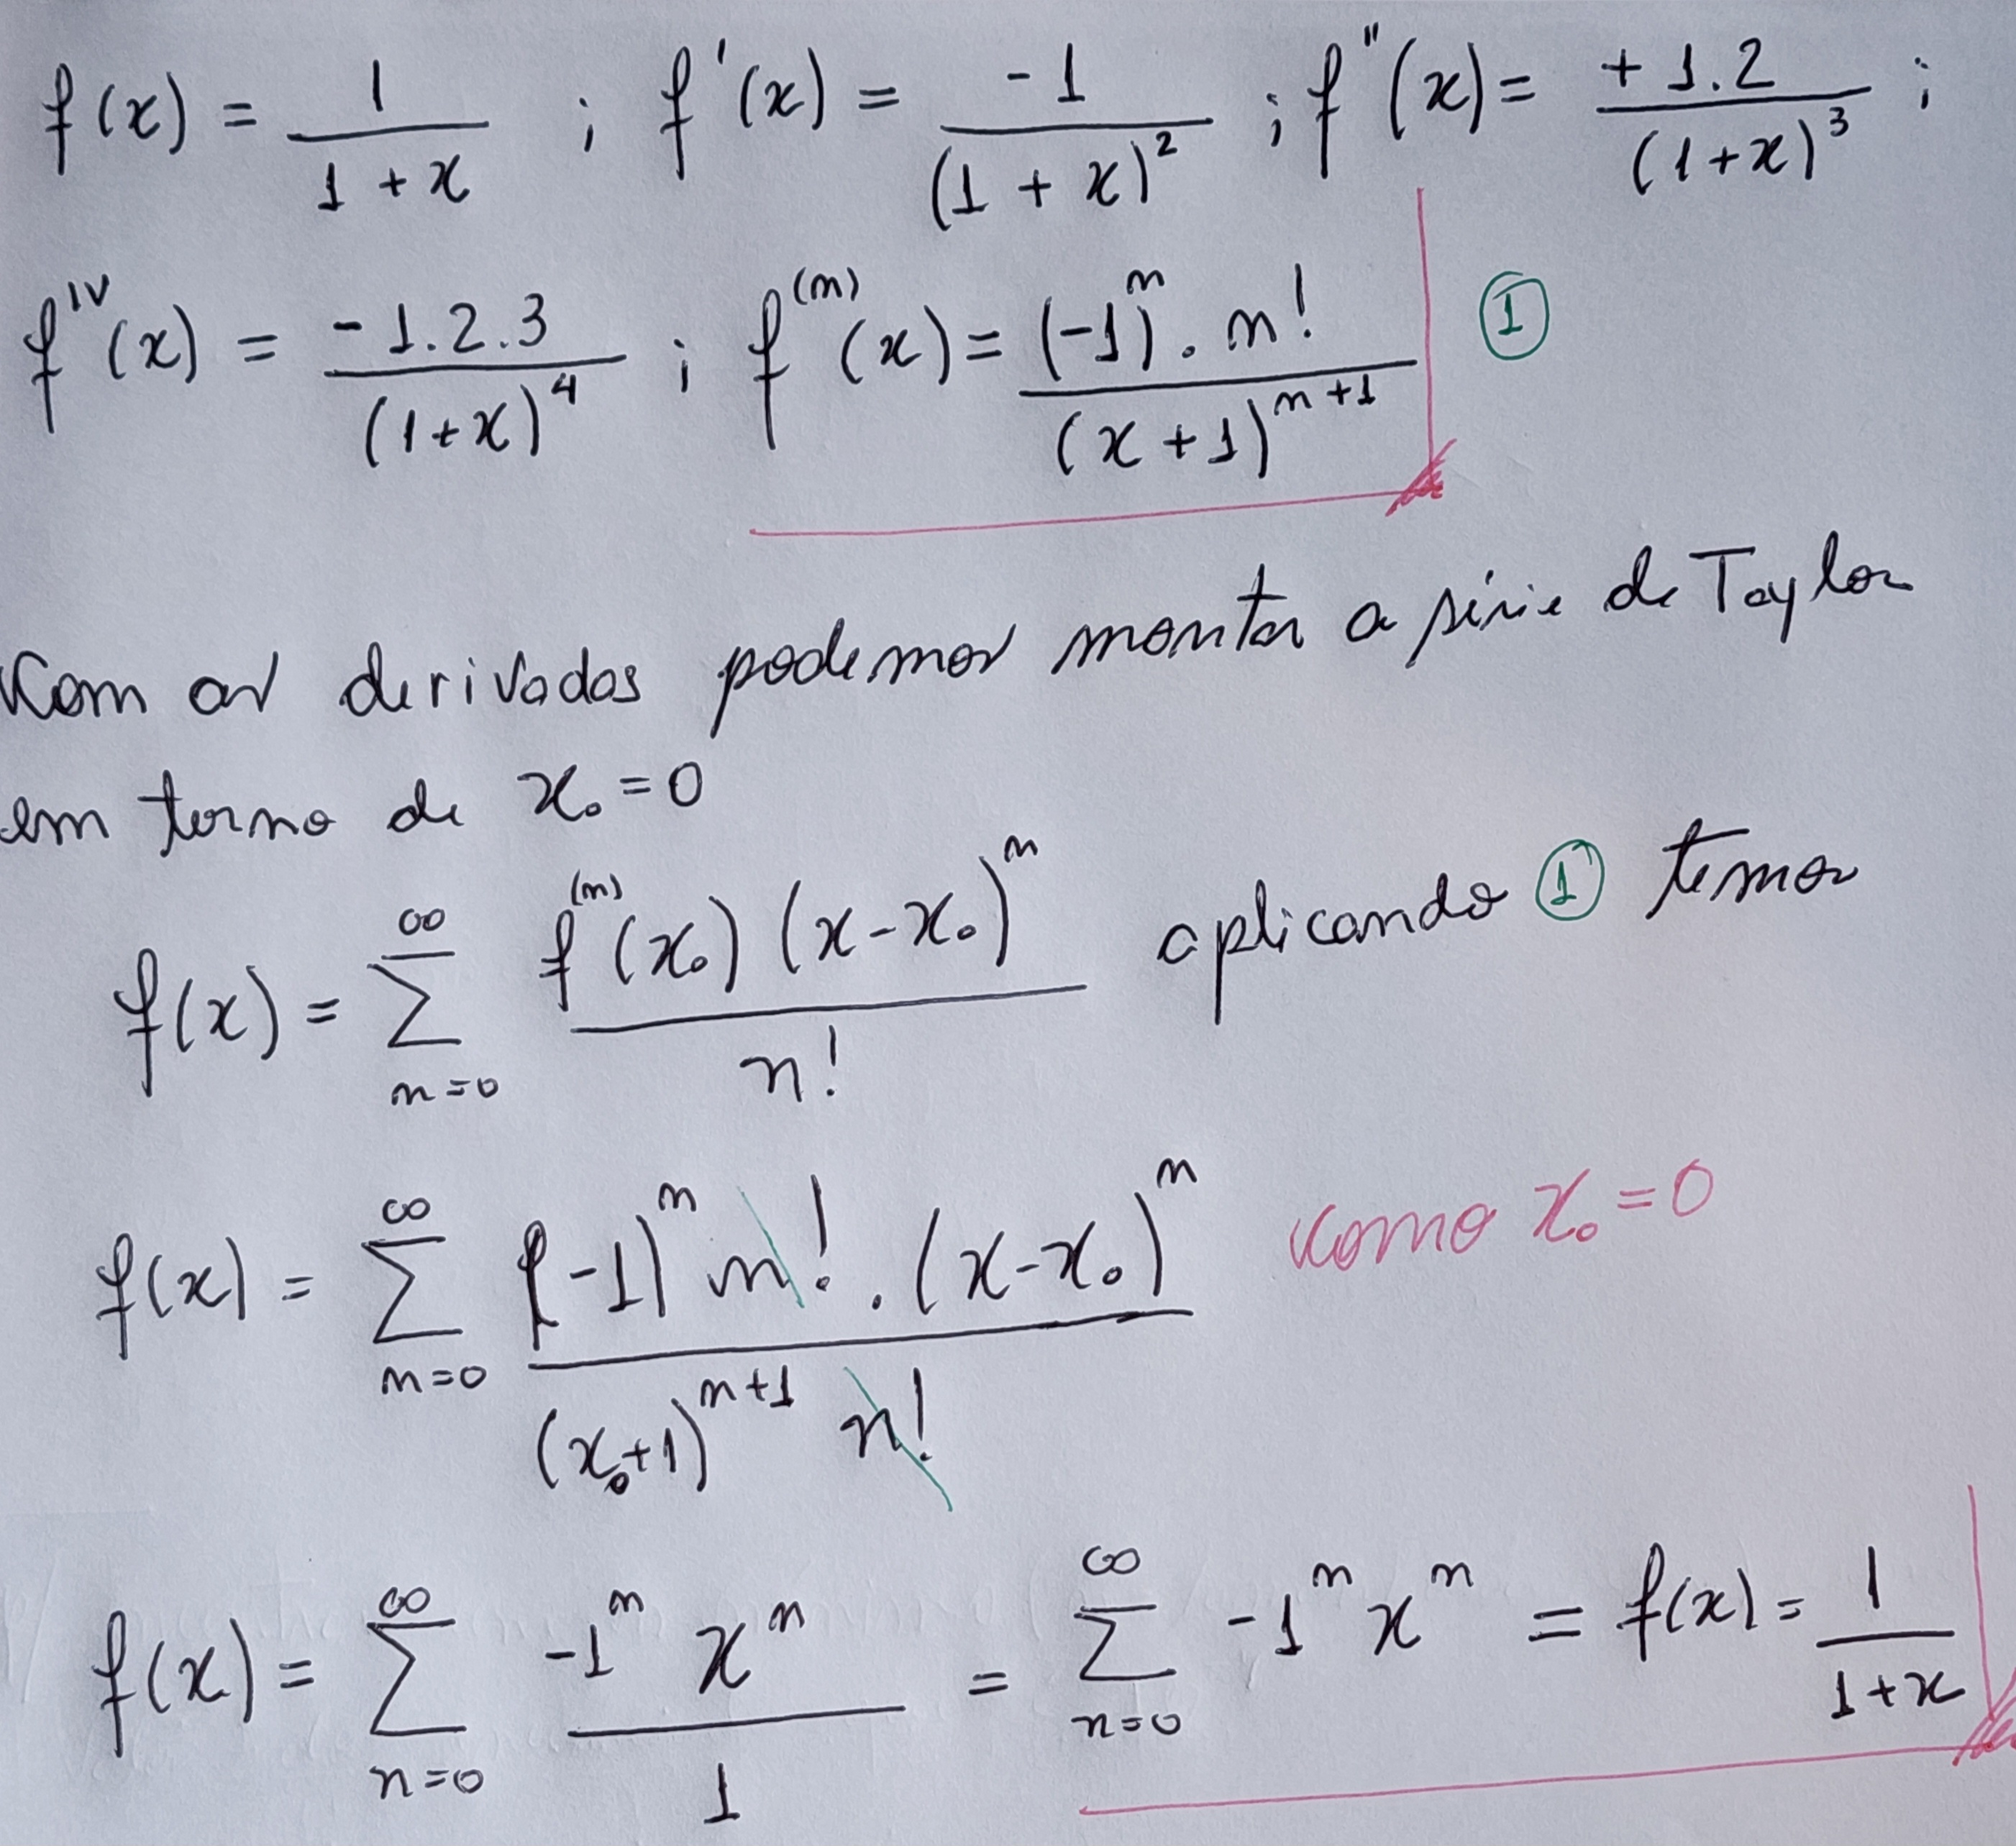
\includegraphics[width=1.1\textwidth]{imagens/exercicio4_parte1}
    \caption{Calculando a série de Taylor de $f(x) = \frac{1}{1 - x}$}
    \label{fig:exe4_parte1}
\end{figure}

\newpage
\subsubsection{Aplicar $t^2$ no resultado}

Ao aplicar $t^2$ em $f(x)$ definida pela série $f(x) = \sum_{n=0}^{\infty} (-1)^n \cdot x^n $ ou escrita na forma:

$f(x) = 1 - x + x^2 - x^3 + x^4 - x^5 \mathellipsis $ \\
Agora teremos como resultado

\begin{figure}[H]
    \centering
    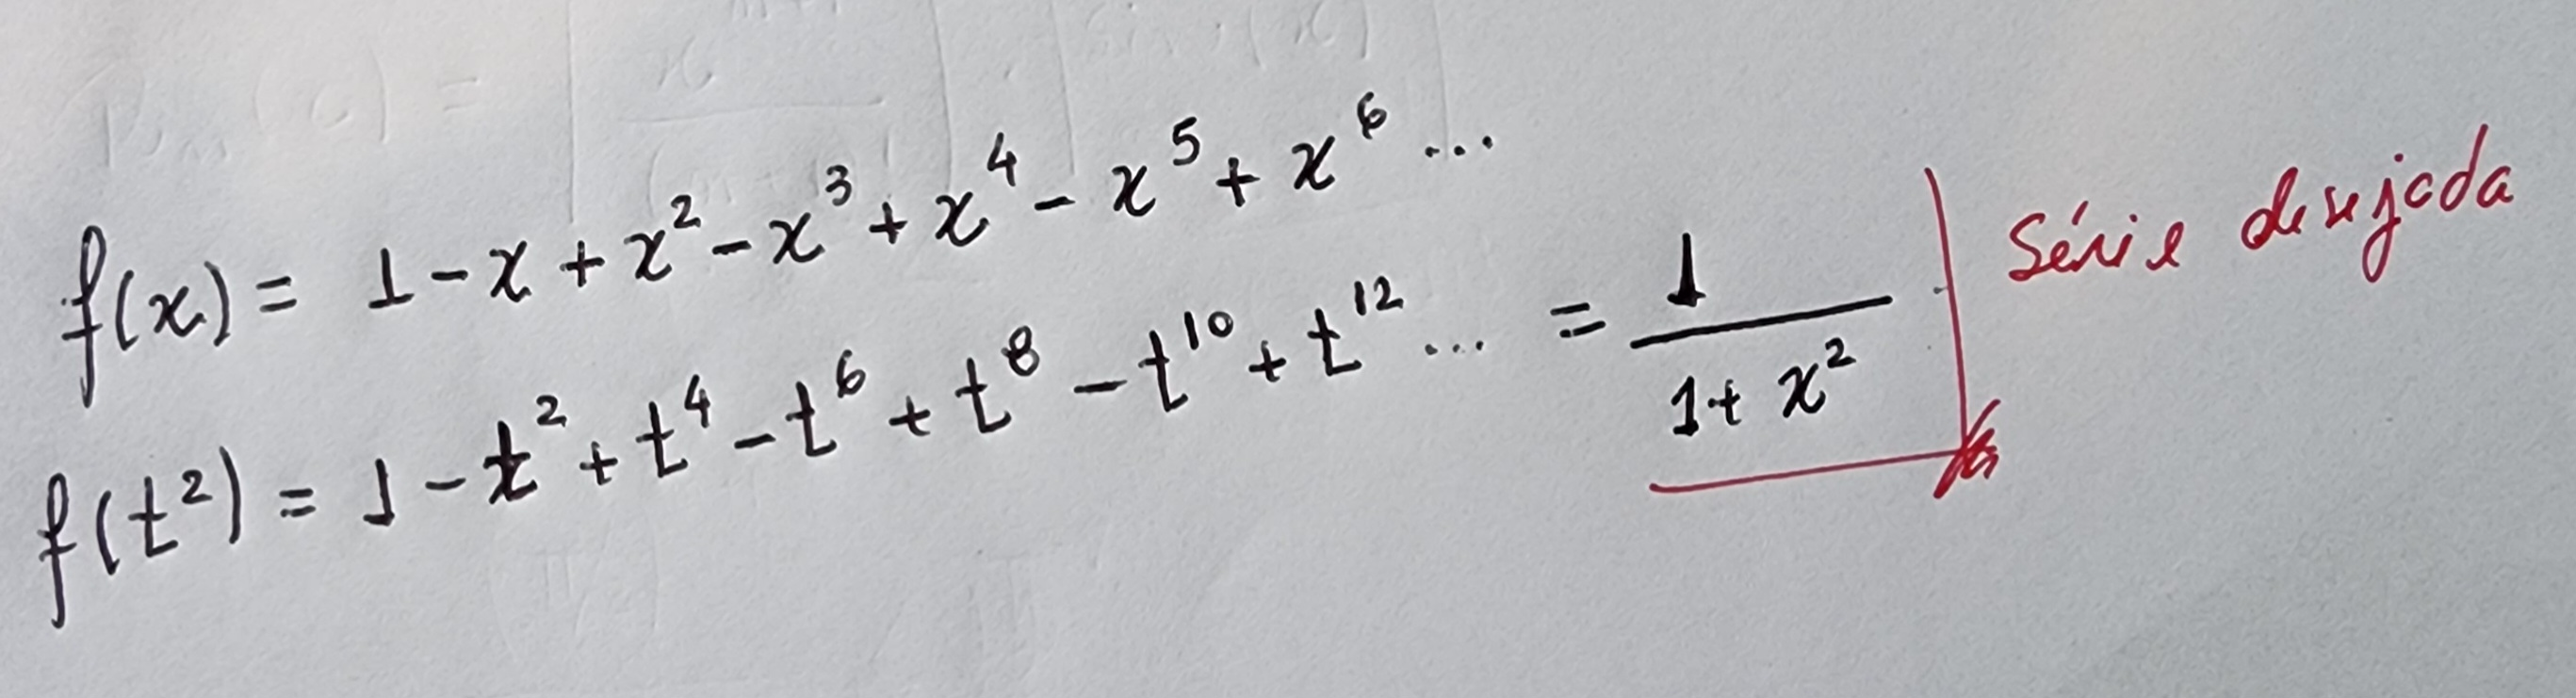
\includegraphics[width=1.0\textwidth]{imagens/exercicio4_parte2}
    \caption{Calculando a série de Taylor desejada $f(x) = \frac{1}{1 - x^2}$}
    \label{fig:exe4_parte2}
\end{figure}

A Figura~\ref{fig:exe4_parte2} mostra que o resultado da expansão usando a série de Taylor para $f(t) = \frac{1}{1 + t^2}$ é

$f(t) = \sum_{n=0}^{\infty} (-1)^n \cdot t^{2 \cdot n}$

\subsubsection{Comparar e aplicar com a função $f(x) = arctan(x)$}

\begin{figure}[H]
    \centering
    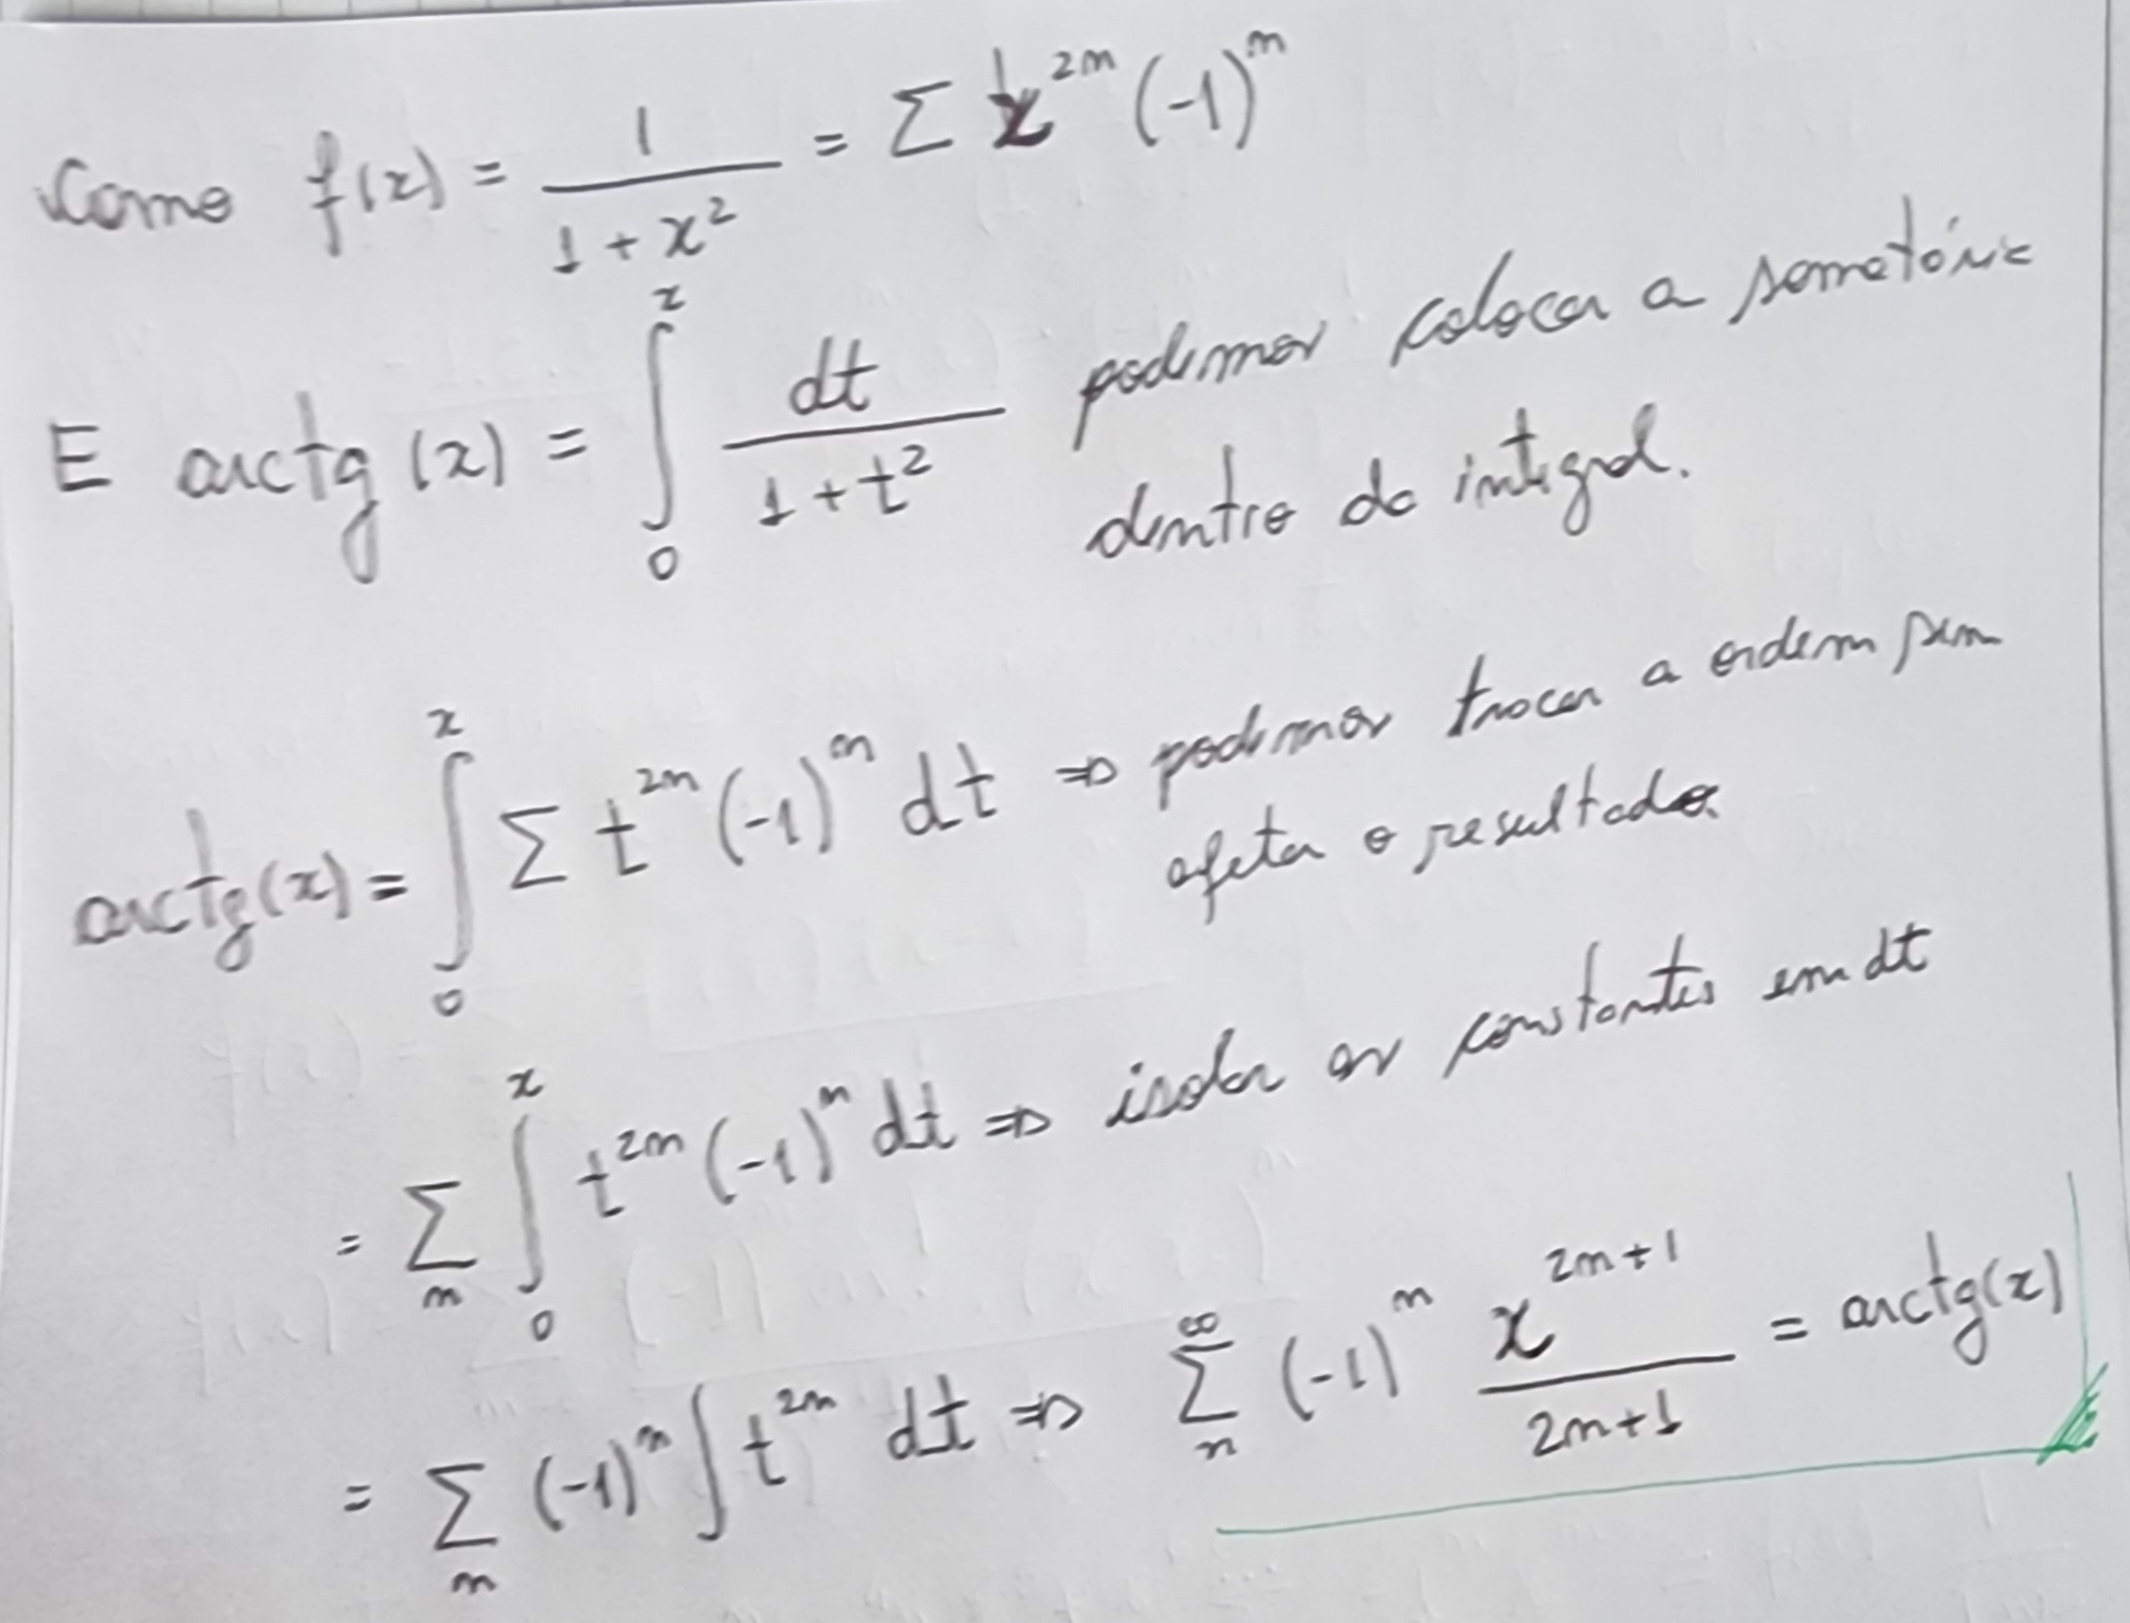
\includegraphics[width=1.0\textwidth]{imagens/exercicio4_parte3}
    \caption{Calculando a série de Taylor para $f(x) = arctan(x)$}
    \label{fig:exe4_parte3}
\end{figure}

Assim temos que $f(x) = arctan(x) = x + \frac{-x^3}{3} + \frac{x^5}{5} + \mathellipsis + \frac{(-1)^n \cdot x^{2 \cdot n + 1}}{2 \cdot n + 1} $

\subsubsection{Problemas com a série}

Foi implementado a série usando o algoritmo de Hormer com sucesso, no entando, para valores acima de um $(1.0)$ a série diverge.
Isso causa um erros consideráveis. Parar evitar esse problema utilizamos relações trigonométricas do site \cite{site-geek} para manter o valor de x menor que 1.

Isso foi colocado no código na função \texttt{calcula\_f\_x\_taylor\_com\_horner\_ajustado}. Está sendo utilizado algumas características do \texttt{arctan} para ficarmos entre $0.$ e $1.$ além das simetrias de uma função impar.

\subsubsection{Melhoramentos para redução das diferenças}
\label{sec:melhoramentos-serie-arctan}
Foi usado a caractéricas que $arctan(-x) = -arctan(x)$. Essa característica mantém os valores de $x$ sempre no domínio positivo.\\
Outra característica foi usada para manter o domínio de x entre 0 e 1 que foi:
\begin{itemize}
    \item[] $\arctan\left(\frac{1}{x}\right) = \frac{\pi}{2} - \arctan(x) = \mathrm{arccot}(x), \quad \text{se } x > 0$
\end{itemize}

O resultado final dos ajustes está na Tabela~\ref{tab:exercicio_4_resultados} e são muito significativos.\\

Executando o programa com 60 mil valores de $-300$ a $+299.99$ temos:

\begin{table}[h!]
    \centering
    \caption{Quadro comparativo com valores entre $-300$ e $299.99$ com séria de $arctan(x)$ usando e não usando ajuste considerado em \cite{site-geek}}
    \label{tab:exercicio_4_critica_1}
    \begin{tabular}{|c|c|c|c|c|}
        \hline
        \textbf{Tipo} & \textbf{Quantidade Total} & \textbf{Erros $>1\%$} & \textbf{Erros $<1\%$} & \textbf{Intervalo com erro $>1 \%$} \\
        \hline
        Com Ajuste & 60.000 & 11 & 59.989 & [0.95 , 1.05] \\
        Sem Ajuste & 60.000 & 29906 & 30095 & [0.95 , 300.] \\
        \hline
    \end{tabular}
\end{table}

Analisando os intervalos de valores com erro segundo Tabela~\ref{tab:exercicio_4_critica_1}, os 11 valores com erro maior que $1 \%$ ficam entre $0.95$ e $1.05$.\\
Ao contrário do que acontece quando não realizamos o ajuste que tem uma quantidade que é praticamente $50 \%$ dos itens que tem o módulo entre 0.95 e 300.\\
Assim, o ajuste foi muito eficiente e reduz substancialmente a quantidade de erros devido a convergência da série usada.

\subsubsection{Apresentação dos testes solicitados}
    
    \begin{table}[h!]
    \centering
    \caption{Testes do Exercicio 4}
    \label{tab:exercicio_4_resultados}
    \begin{tabular}{|c|c|c|c|c|c|}
    \toprule
    \textbf{$x$} & \textbf{$f(x)$ (NP)} & \textbf{$P_{10}(x)$  s/ ajuste} & \textbf{$P_{10}(x)$ c/ ajuste} & \textbf{Dif. sem ajuste} & \textbf{Dif. com ajuste}\\
    \midrule
    
    1.5708e+00 & 1.0039e+00 & -1.9211e+02 & 1.0039e+00& 1.9311e+02 & 2.6472e-06 \\
                          1.0472e+00 & 8.0845e-01 & 7.4565e-01 & 8.1833e-01& 6.2802e-02 & 9.8820e-03 \\
                          7.8540e-01 & 6.6577e-01 & 6.6558e-01 & 6.6558e-01& 1.9103e-04 & 1.9103e-04 \\
                          
    \bottomrule
    \end{tabular}
    \end{table}    
    

\subsubsection{Apresentar o código Python}
    \lstinputlisting[style=python]{scripts/exercicio4.py}
    Código para solução e testes do exercício 4.


        \section{Conclusão}
A integração entre Java, Gnuplot e LaTeX oferece uma abordagem poderosa e flexível para automação de relatórios científicos.
%\chapter{Conclusão}
A automação com Gradle, Java, Gnuplot e \LaTeX mostrou-se eficaz e escalável. O modelo pode ser aplicado a diversas áreas científicas.


        \bibliography{referencias}
\end{document}

